\documentclass[
	12pt,
	openright,
	twoside,
	a4paper,
	brazil,
]{abntex2}

% -----------------------------------------------------------------------------
% PACOTES
% -----------------------------------------------------------------------------

\usepackage{cmap}
\usepackage{lmodern}
\usepackage[T1]{fontenc}
\usepackage[utf8]{inputenc}
\usepackage{lastpage}
\usepackage{indentfirst}
\usepackage{color}
\usepackage{graphicx}
\usepackage{lipsum}
\usepackage[brazilian,hyperpageref]{backref}
\usepackage[alf]{abntex2cite}
\usepackage[table,xcdraw]{xcolor}
\usepackage{tabularray}
\usepackage{longtable}

% ------------------------------------------------------------------------------------------------
% JSON
\usepackage{listings,xcolor,caption}
\colorlet{punct}{red!60!black}
\definecolor{background}{HTML}{EEEEEE}
\definecolor{delim}{RGB}{20,105,176}
\colorlet{numb}{magenta!60!black}

\lstdefinelanguage{json}{
    basicstyle=\normalfont\ttfamily,
    numbers=left,
    numberstyle=\scriptsize,
    stepnumber=1,
    numbersep=8pt,
    showstringspaces=false,
    breaklines=true,
    frame=lines,
    backgroundcolor=\color{background},
    literate=
     *{0}{{{\color{numb}0}}}{1}
      {1}{{{\color{numb}1}}}{1}
      {2}{{{\color{numb}2}}}{1}
      {3}{{{\color{numb}3}}}{1}
      {4}{{{\color{numb}4}}}{1}
      {5}{{{\color{numb}5}}}{1}
      {6}{{{\color{numb}6}}}{1}
      {7}{{{\color{numb}7}}}{1}
      {8}{{{\color{numb}8}}}{1}
      {9}{{{\color{numb}9}}}{1}
      {:}{{{\color{punct}{:}}}}{1}
      {,}{{{\color{punct}{,}}}}{1}
      {\{}{{{\color{delim}{\{}}}}{1}
      {\}}{{{\color{delim}{\}}}}}{1}
      {[}{{{\color{delim}{[}}}}{1}
      {]}{{{\color{delim}{]}}}}{1},
}

\renewcommand{\lstlistingname}{Bloco de Código} % Listing -> Bloco de Código
\renewcommand{\lstlistlistingname}{Lista de Blocos de Código} % List of Listings -> Lista de Blocos de Código

% ------------------------------------------------------------------------------------------------

\renewcommand{\backrefpagesname}{Citado na(s) página(s):~}
\renewcommand{\backref}{}
\renewcommand*{\backrefalt}[4]{
    \ifcase #1 %
        Nenhuma citação no texto.%
    \or
        Citado na página #2.%
    \else
        Citado #1 vezes nas páginas #2.%
    \fi}%
% -----------------------------------------------------------------------------


% -----------------------------------------------------------------------------
% Informações de dados para CAPA e FOLHA DE ROSTO
% -----------------------------------------------------------------------------
\titulo{Protótipo de um nó IoT acionado pela Amazon Alexa e integrado ao serviço AWS IoT}
\autor{Guilherme Vinícius Barbosa Pereira Amorim}
\local{Belo Horizonte}
\data{2022}
\orientador{Prof. Ricardo de Oliveira Duarte}
\instituicao{%
  Universidade Federal de Minas Gerais -- UFMG
  \par
  Escola de Engenharia
  \par
  Curso de Graduação em Engenharia Elétrica}
\tipotrabalho{Trabalho de Conclusão de Curso}

% O preambulo deve conter o tipo do trabalho, o objetivo, o nome da instituição e a área de concentração
\preambulo{Monografia apresentada durante o Seminário dos Trabalhos de Conclusão do Curso de Graduação em Engenharia Elétrica da UFMG, como parte dos requisitos necessários à obtenção do título de Engenheiro Eletricista.}
% -----------------------------------------------------------------------------

% -----------------------------------------------------------------------------
% Configurações de aparência do PDF final

% alterando o aspecto da cor azul
\definecolor{blue}{RGB}{41,5,195}

% informações do PDF
\makeatletter
\hypersetup{
        pdftitle={\@title},
        pdfauthor={\@author},
        pdfsubject={\imprimirpreambulo},
        pdfcreator={LaTeX with abnTeX2},
        pdfkeywords={abnt}{latex}{abntex}{abntex2}{trabalho acadêmico},
        colorlinks=true,
        linkcolor=blue,
        citecolor=blue,
        filecolor=magenta,
        urlcolor=blue,
        bookmarksdepth=4
}
\makeatother
% -----------------------------------------------------------------------------

% -----------------------------------------------------------------------------
% Espaçamentos entre linhas e parágrafos
% -----------------------------------------------------------------------------

% O tamanho do parágrafo é dado por:
\setlength{\parindent}{1.3cm}

% Controle do espaçamento entre um parágrafo e outro:
\setlength{\parskip}{0.2cm}

% -----------------------------------------------------------------------------
% compila o índice
% -----------------------------------------------------------------------------
\makeindex
% -----------------------------------------------------------------------------

% ----
% Início do documento
% ----
\begin{document}

% Retira espaço extra obsoleto entre as frases.
\frenchspacing

% -----------------------------------------------------------------------------
% ELEMENTOS PRÉ-TEXTUAIS
% -----------------------------------------------------------------------------
% \pretextual

% -----------------------------------------------------------------------------
% Capa
% -----------------------------------------------------------------------------
\imprimircapa
% -----------------------------------------------------------------------------

% -----------------------------------------------------------------------------
% Folha de rosto
% -----------------------------------------------------------------------------
\imprimirfolhaderosto
% -----------------------------------------------------------------------------

% -----------------------------------------------------------------------------
% Dedicatória
% -----------------------------------------------------------------------------
\begin{dedicatoria}
\end{dedicatoria}
% -----------------------------------------------------------------------------

% -----------------------------------------------------------------------------
% Agradecimentos
% -----------------------------------------------------------------------------
\begin{agradecimentos}
\end{agradecimentos}
% -----------------------------------------------------------------------------

% -----------------------------------------------------------------------------
% inserir lista de ilustrações
% -----------------------------------------------------------------------------
\pdfbookmark[0]{\listfigurename}{lof}
\listoffigures*
\cleardoublepage
% -----------------------------------------------------------------------------

% -----------------------------------------------------------------------------
% inserir lista de tabelas
% -----------------------------------------------------------------------------
\pdfbookmark[0]{\listtablename}{lot}
\listoftables*
\cleardoublepage
% -----------------------------------------------------------------------------

% -----------------------------------------------------------------------------
% inserir lista de blocos de código
% -----------------------------------------------------------------------------
\pdfbookmark[0]{\lstlistlistingname}{lot}
\lstlistoflistings
\cleardoublepage
% -----------------------------------------------------------------------------

% -----------------------------------------------------------------------------
% inserir lista de tabelas
% -----------------------------------------------------------------------------
\begin{siglas}
    \item[ASK] Alexa Skills Kit
    \item[AWS] Amazon Web Services
    \item[CLI] AWS Command Line Interface
    \item[EC2] Amazon Elastic Compute Cloud
    \item[HTTPS] Hypertext Transfer Protocol Secure
    \item[IAM] AWS Identity and Access Management
    \item[IDE] Ambiente de desenvolvimento integrado
    \item[IoT] Internet das Coisas
    \item[LED] Diodo emissor de luz
    \item[MQTT] MQ Telemetry Transport
    \item[SDK] Kit de desenvolvimento de software
    \item[TI] Tecnologia da Informação
    \item[TLS] Transport Layer Security
    \item[USB] Universal Serial Bus
\end{siglas}

% -----------------------------------------------------------------------------
% inserir o sumario
% -----------------------------------------------------------------------------
\pdfbookmark[0]{\contentsname}{toc}
\tableofcontents*
\cleardoublepage
% -----------------------------------------------------------------------------

% -----------------------------------------------------------------------------
% ELEMENTOS TEXTUAIS
% -----------------------------------------------------------------------------
\textual

% -----------------------------------------------------------------------------
% Capítulo 1 - Introdução
% -----------------------------------------------------------------------------
\chapter{Introdução}\label{chapter:introducao}

Computação em nuvem é um termo que surgiu na década de 1960 com os sistemas de compartilhamento de tempo. Atualmente, define-se computação em nuvem como a entrega de recursos de TI através da Internet e sob demanda com definição de preço conforme o uso \cite{ref:000}. Dessa forma, empresas e usuários de tecnologia conseguem expandir seus negócios de maneira rápida e estratégica sem ter que se preocupar com uma infraestrutura própria de TI. Algumas empresas que fornecem serviço de computação em nuvem são: AWS, Google Cloud Platform, Microsoft Azure e IBM Cloud.

Dessa maneira, a nuvem oferece agilidade, elasticidade e economia de custos para organizações de todos os tipos, portes e setores. Esse tipo de tecnologia permite a geração rápida de recursos de acordo com a evolução das necessidades empresariais. Assim, empresas que fazem uso de computação em nuvem não correm o risco de provisionar recursos em excesso para absorver picos de atividades empresariais futuras. Por fim, a nuvem permite a troca de despesas fixas, como \textit{datacenters}, segurança de dados e servidores públicos, por despesas variáveis que dependem somente do que foi consumido \cite{ref:000}.

% Atualmente o termo "sistemas embarcados" não está muito presente no cotidiano brasileiro, mas essa tecnologia é responsável por fornecer equipamentos inteligentes como semáforos de trânsito, relógios, respiradores mecânicos, roteadores e aparelhos de ar-condicionado, por exemplo. Em termos simples, pode-se definir um sistema embarcado como um dispositivo controlado por um computador encapsulado. Ou seja, um sistema embarcado é na verdade um sistema microprocessado. Dentre as principais vantagens de sistemas embarcados, destaca-se o baixo custo, a eficiência e a facilidade de programação (NORLETO, 2020).

% O primeiro sistema embarcado é o AGC (Apollo Guidance Computer). Ele foi desenvolvido nos EUA por Charles Stark Draper do MIT em 1966 (EMBARCADOS, 2014). Desde então, os sistemas embarcados ficaram mais acessíveis, mais velozes e mais compactos.

% Com o passar dos anos, novas tecnologias foram adicionadas à sistemas embarcados, como por exemplo o Wifi, o Bluetooth etc. Na última década foi observado a ascensão de assistentes virtuais como a Alexa e o Google Assistente. A Alexa foi criada em 2014 e apareceu pela primeira vez como parte das caixas de som. Hoje a Alexa, a partir de comandos de voz, pode realizar pesquisas, mandar executar uma lista de músicas, disparar um alarme etc.(VIGLIAROLO, 2017). Segundo o site oficial da Alexa (2022), o serviço permite a conexão com dispositivos, efetuar comandos por voz, interpretá-los e tomar uma ação correspondente. Isso tudo acontece por meio da AWS.

Já o termo Internet das Coisas, ou simplesmente IoT, surgiu em 1999 com um sistema de sensores omnipresentes conectados à internet. A tecnologia ganhou popularidade e se expande com o crescimento de tecnologias de conectividade, computação em nuvem e aprendizado de máquina, por exemplo. Uma definição simplificada de IoT é: uma rede de itens conectados à internet. A principal vantagem dessa tecnologia é a não intervenção humana, o que gera um aumento na produtividade de tarefas repetitivas e escalabilidade.

Outra tecnologia recente são as assistentes virtuais inteligentes. Uma assistente virtual inteligente é um agente de software que pode realizar tarefas ou serviços para um indivíduo. Algumas informações que as assistentes são capazes de acessar e rapidamente leva-las ao usuário, em linguagem natural, são: notícias, condições meteorológicas e de trânsito, agenda do usuário, entre outras. Alguns exemplos disponíveis no mercado são a Alexa, Microsoft Cortana, Siri e Google Assistant \cite{ref:001}.

Em 25 de setembro de 2019, o Alexa e o Google Assistant puderam ajudar seus usuários a se candidatarem a empregos no McDonald's usando serviços de reconhecimento de voz. É o primeiro serviço de emprego do mundo usando o serviço de comando de voz. A Amazon anunciou em 25 de setembro de 2019 que Alexa em breve poderá imitar vozes de celebridades, incluindo Samuel L. Jackson, custando US \$ 0,99 para cada voz \cite{ref:002}.

Dessa forma, uma tendência das tecnologias focadas na experiência do usuário, como a IoT, é o suporte às assistentes virtuais. Diante do que foi dito, este trabalho propõe criar um prototipo de um nó IoT integrado à assistente de voz Alexa e serviços em nuvem.

\section{Estrutura}
O trabalho será apresentado em cinco capítulos. O \autoref{chapter:introducao} apresenta a introdução, contexto histórico e a motivação do projeto. O \autoref{chapter:referencial_teorico} apresenta o referencial teórico e trabalhos correlatos. O \autoref{chapter:metodologia} contém o desenvolvimento do trabalho, apresentando requisitos funcionais e não-funcionais, ferramentas utilizadas e o processo de desenvolvimento. O \autoref{chapter:resultados_e_discussoes} faz a análise dos resultados. O \autoref{chapter:conclusoes}, por fim, conclui o trabalho, listando dificuldades enfrentadas, vantagens, desvantagens e as sugestões para trabalhos futuros. O projeto conta também com o \autoref{chapter:apendice}, que é um capítulo extra de apêndice.


% -----------------------------------------------------------------------------
% Capítulo 2 - Referencial teórico
% -----------------------------------------------------------------------------
\chapter{Referencial teórico}\label{chapter:referencial_teorico}

% -----------------------------------------------------------------------------
% Capítulo 2.1 - IoT
% -----------------------------------------------------------------------------
\section{IoT}

Nos últimos anos, observou-se a ascensão de dispositivos inteligentes, dispositivos que se conectam à Internet. Esses dispositivos se comunicam entre si, possuem sensores e outras tecnologias. Em termos simples, define-se IoT como uma rede de itens - cada um com sensores integrados - que são conectados à Internet \cite{ref:003}.

Aprofundando, IoT também pode ser definido como uma rede que engloba um sistema de dispositivos de computação inter-relacionados, máquinas mecânicas e digitais, objetos, animais ou pessoa, e a capacidade de transferir dados através de uma rede sem a necessidade de interação entre humanos \cite{ref:004}. A presença de tecnologias de nuvem, \textit{big data} e redes móveis, por exemplo, em redes de IoT permite o compartilhamento e a coleta de dados com o mínimo de intervenção humana \cite{ref:005}. Pode-se listar as seguintes tecnologias como as protagonistas no crescimento do uso da tecnologia IoT:

\begin{itemize}
    \item Acesso a tecnologia de sensores de baixo custo e baixa potência;
    \item Conectividade;
    \item Plataformas de computação em nuvem;
    \item Aprendizado de máquina e análise avançada;
    \item Processamento de linguagem natural (Amazon Alexa, por exemplo).
\end{itemize}

Uma característica comum dos dispositivos IoT é a necessidade de componentes de interface para a interação com o mundo físico. Alguns exemplos de componentes de interface são:

\begin{itemize}
    \item Teclado, botões e microfones;
    \item Alarmes, visores e alto-falantes;
    \item Sensores;
    \item Atuadores;
\end{itemize}

% -----------------------------------------------------------------------------
% Capítulo 2.2 - Computação em nuvem com a AWS
% -----------------------------------------------------------------------------
\section{Computação em nuvem com a AWS}

A Amazon Web Services, Inc. (AWS) é uma empresa subsidiária da Amazon responsável por fornecer a seus clientes plataformas para a computação em nuvem sob demanda via Internet. Empresas fazem uso desse serviço para a criação e execução de aplicações virtuais sem um custo inicial, uma vez que a AWS tem o \textit{pay-as-you-go} como modelo de precificação. Ou seja, o cliente faz o pagamento conforme o uso \cite{ref:006}. Em 2022, a AWS é capaz de oferecer a seus clientes mais de duzentos serviços em nuvem nas áreas de tecnologias de computação, banco de dados, \textit{machine learning}, IoT, inteligência artificial etc \cite{ref:007}.

Ademais, a AWS conta com mais de 410 pontos de presença em mais de 90 cidades e 48 países \cite{ref:008}. Esse modelo de região e zona de disponibilidade da AWS foi reconhecido pelo Gartner, empresa de pesquisa e consultoria em TI, como o método recomendado para executar aplicativos corporativos que exigem alta disponibilidade \cite{ref:009}. A \autoref{fig:aws_zone} contém um mapa com as redes de presença da AWS, por região.

\begin{figure}[htbp]
    \centering
    \caption{Redes de presença da AWS.}
    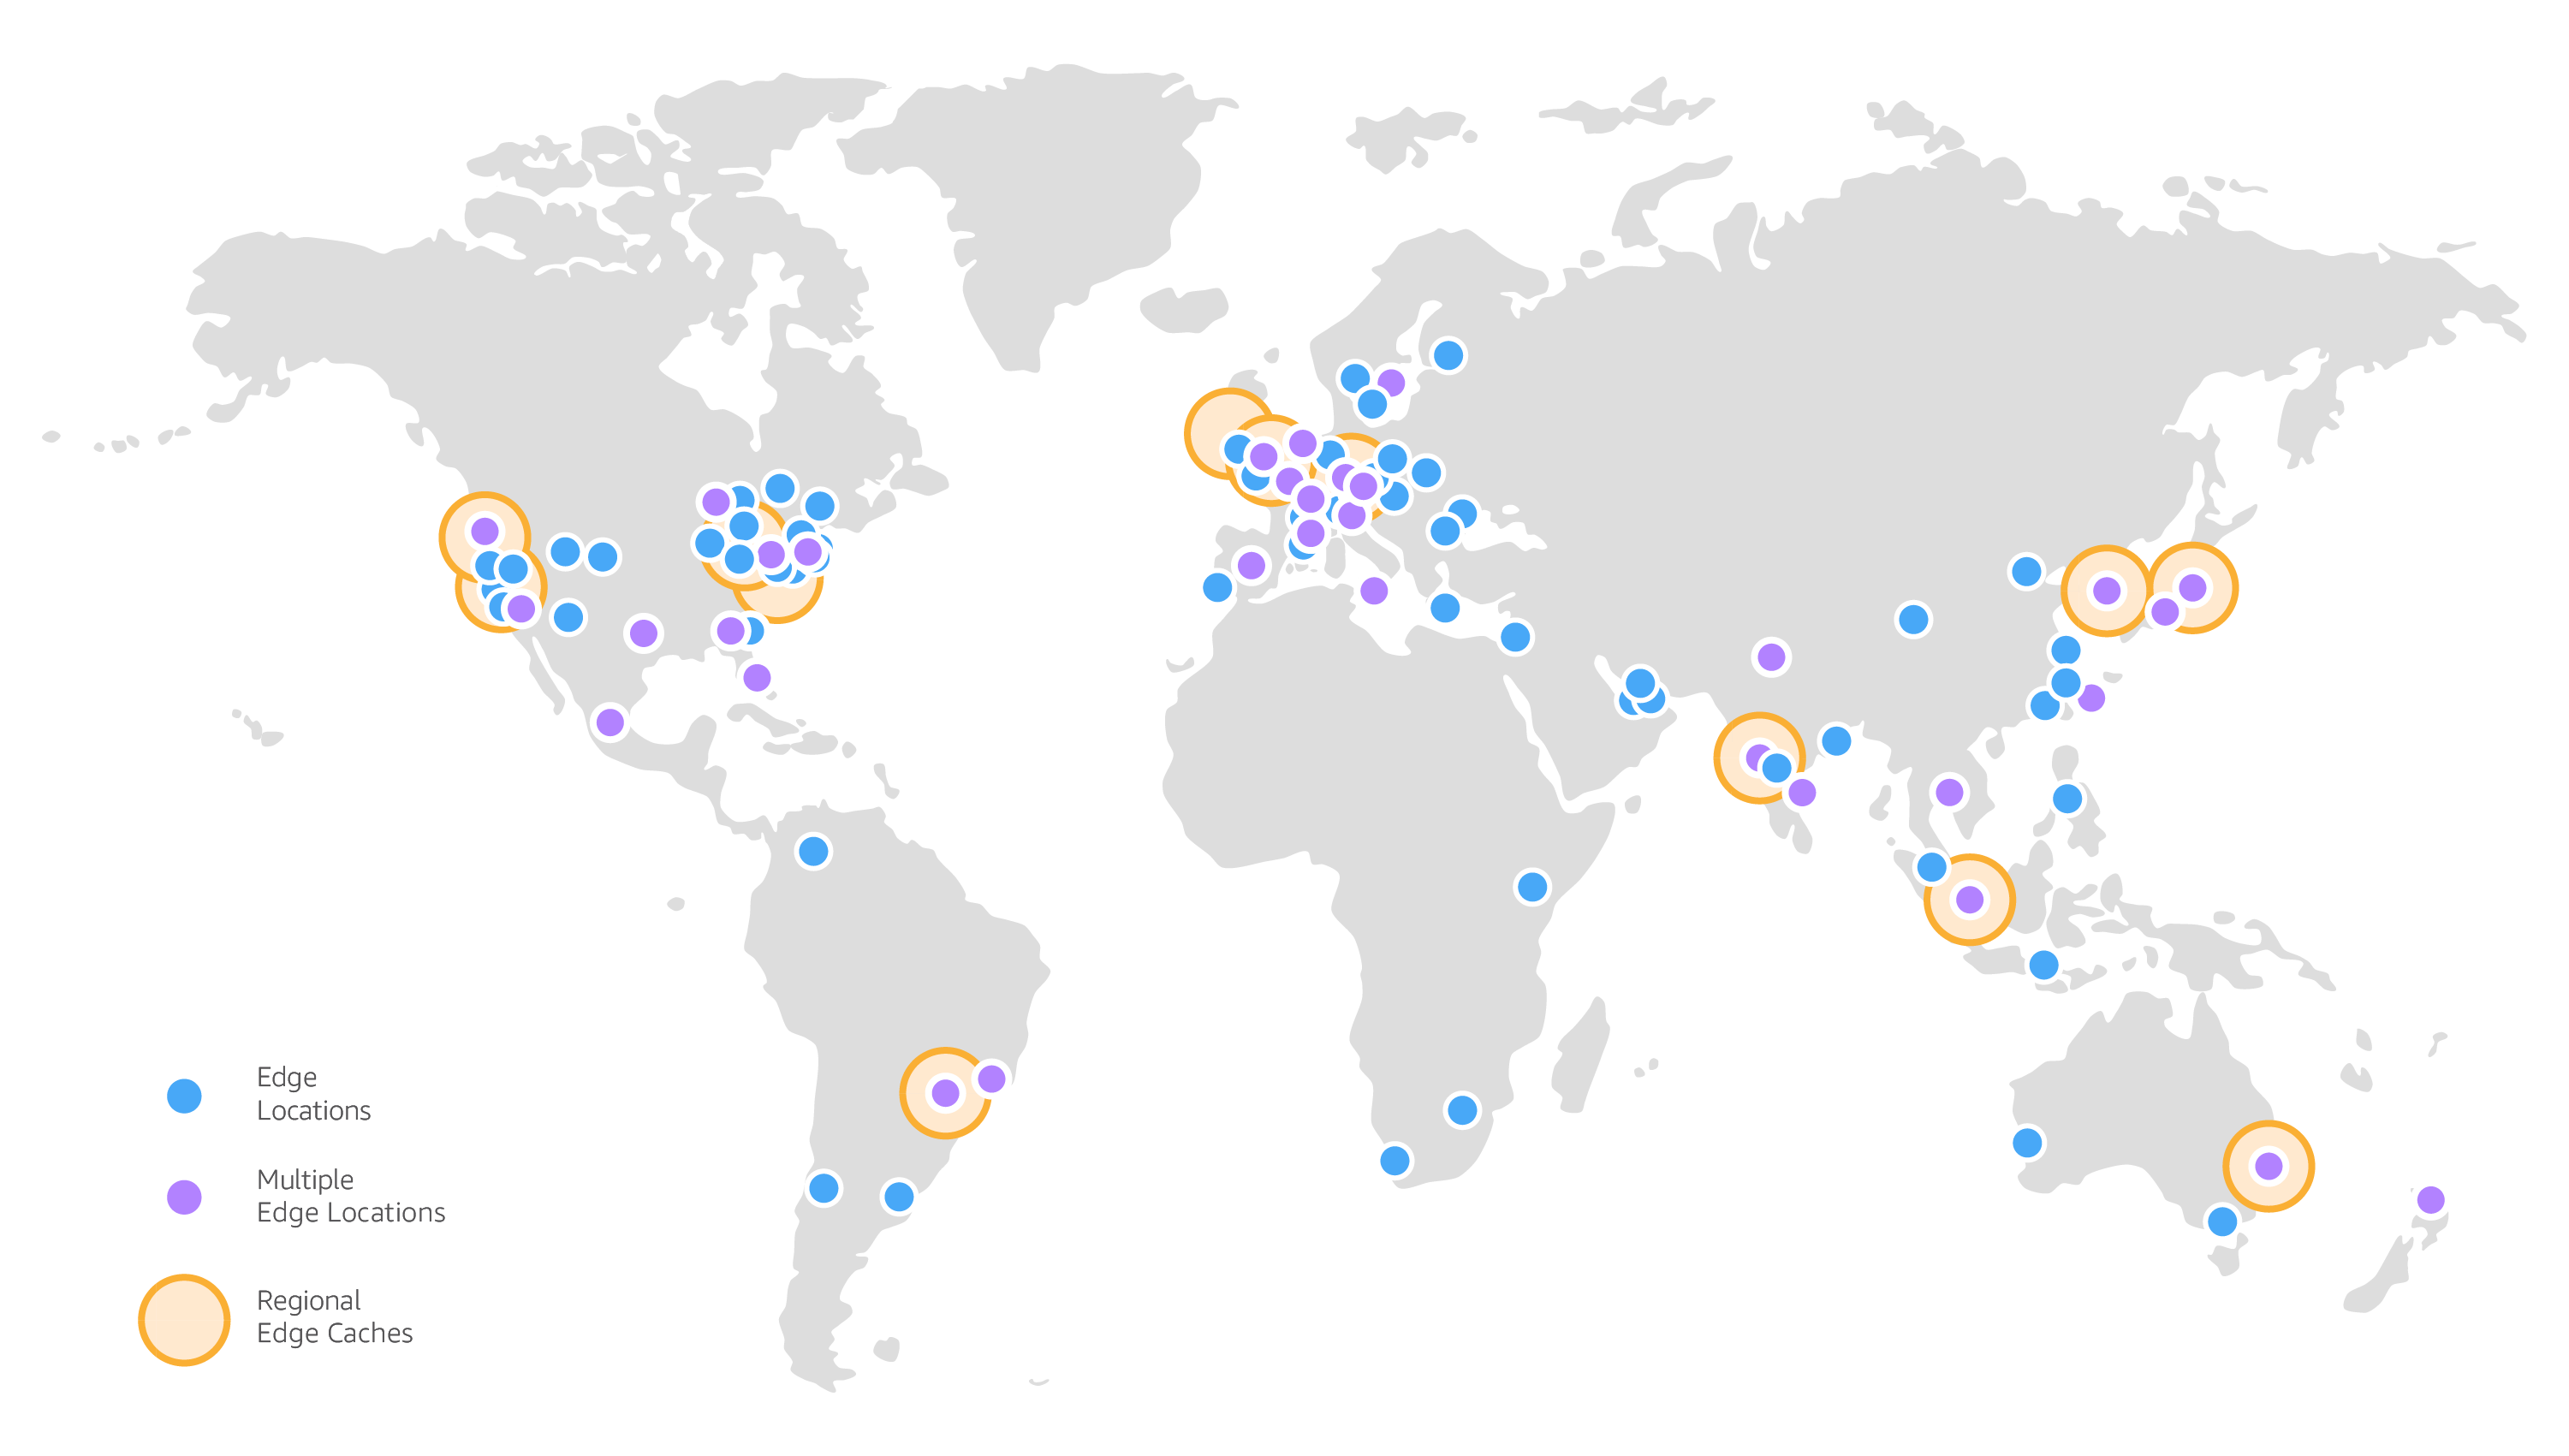
\includegraphics[scale=0.3]{Imagens/aws_zones.png}
    \legend{Fonte: \cite{ref:008}.}
    \label{fig:aws_zone}
\end{figure}

Para o desenvolvimento de aplicações na AWS, a Amazon oferece ao desenvolvedor ferramentas e permite a escolha da linguagem de programação. Destaca-se as seguintes ferramentas:

\begin{itemize}
    \item Console da web;
    \item Ferramenta de linha de comando;
    \item IDE;
    \item SDK;
    \item Infraestrutura como código.
\end{itemize}

% -----------------------------------------------------------------------------
% Capítulo 2.3 - AWS IAM
% -----------------------------------------------------------------------------
\section{AWS IAM}

O AWS IAM é um serviço da Amazon que gerencia e controla o acesso aos recursos da AWS. Com o IAM, o usuário controla de maneira centralizada quem é autenticado (conectado) e autorizado (tem permissões) para usar recursos \cite{ref:010}.

Ao criar uma conta AWS, uma identidade de login é iniciada. Essa identidade é chamada de usuário raiz da conta AWS e tem acesso completo a todos os serviços e recursos. O usuário raiz, contudo, não é recomendado em tarefas diárias. Recomenda-se que usuários tenham um privilégio mínimo e refinado para as suas tarefas.

Ademais, o IAM oferece um controle de acesso baseado em atributos, o que permite a criação de permissões baseadas em particularidades (como departamento, cidade e nome da equipe) \cite{ref:011}.

A \autoref{fig:iam_diagram} apresenta um diagrama detalhando o funcionamento do serviço AWS IAM.

\begin{figure}[htb]
    \centering
    \caption{Diagrama do serviço AWS IAM.}
    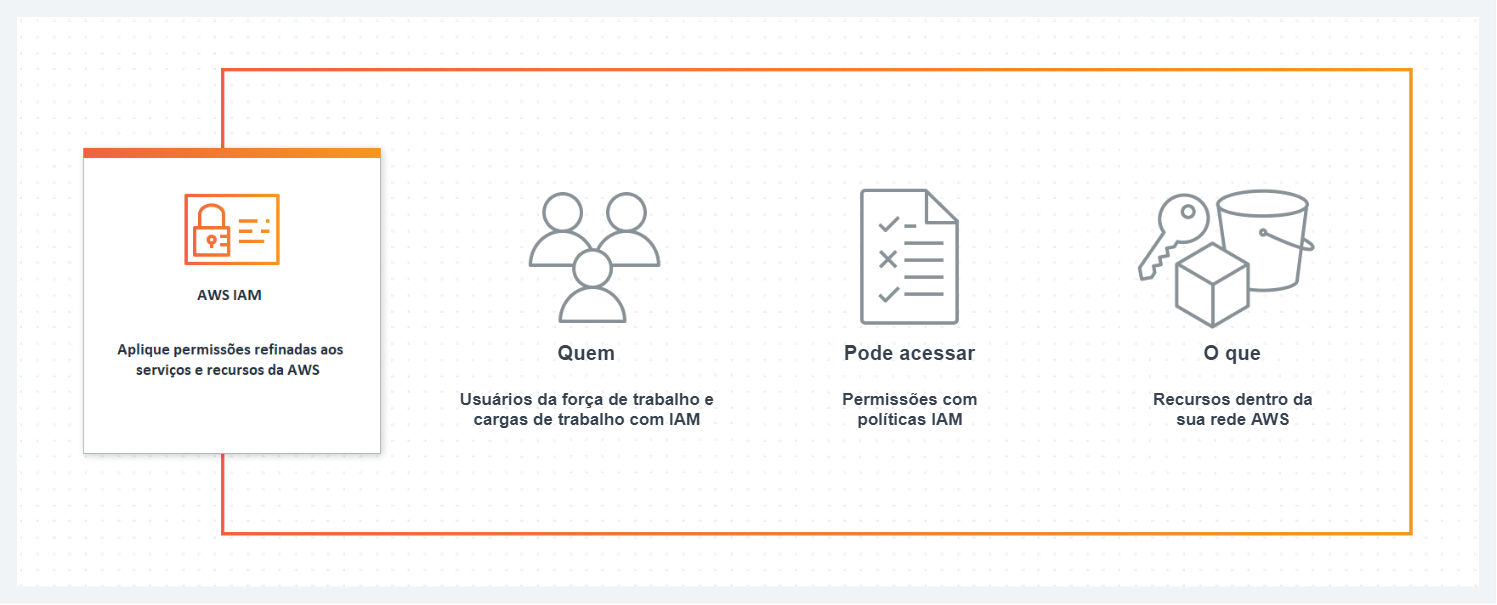
\includegraphics[scale=0.3]{Imagens/iam_diagram.png}
    \legend{Fonte: \cite{ref:011}, com edições feitas pelo autor.}
    \label{fig:iam_diagram}
\end{figure}

% -----------------------------------------------------------------------------
% Capítulo 2.4 - Segurança
% -----------------------------------------------------------------------------
\section{Segurança}\label{section:aws_iot_security}

A AWS adota um modelo de responsabilidade compartilhada de segurança e conformidade entre a AWS e o cliente. Esse modelo tem como principais conceitos o que a Amazon chama de ``segurança da nuvem'' e ``segurança na nuvem'' \cite{ref:012}.

A ``segurança da nuvem'' define que a AWS é responsável por prover serviços seguros proteger a infraestrutura que executa todos os serviços oferecidos na Nuvem AWS. Já a ``segurança na nuvem'' é definida pelo serviço da AWS que o cliente estiver usando. Por exemplo, o serviço Amazon EC2 exige que o cliente execute todas as tarefas necessárias de configuração e gerenciamento da segurança. o cliente também é responsável por fatores como a sensibilidade dos dados, os requisitos da empresa e aplicáveis leis e regulações \cite{ref:013}. A \autoref{fig:modelo_compartilhado_de_responsabilidade} mostra um diagrama oferecido pela AWS que descreve o modelo compartilhado de responsabilidade.

\begin{figure}[htbp]
    \centering
    \caption{Modelo Compartilhado de Responsabilidade de Amazon.}
    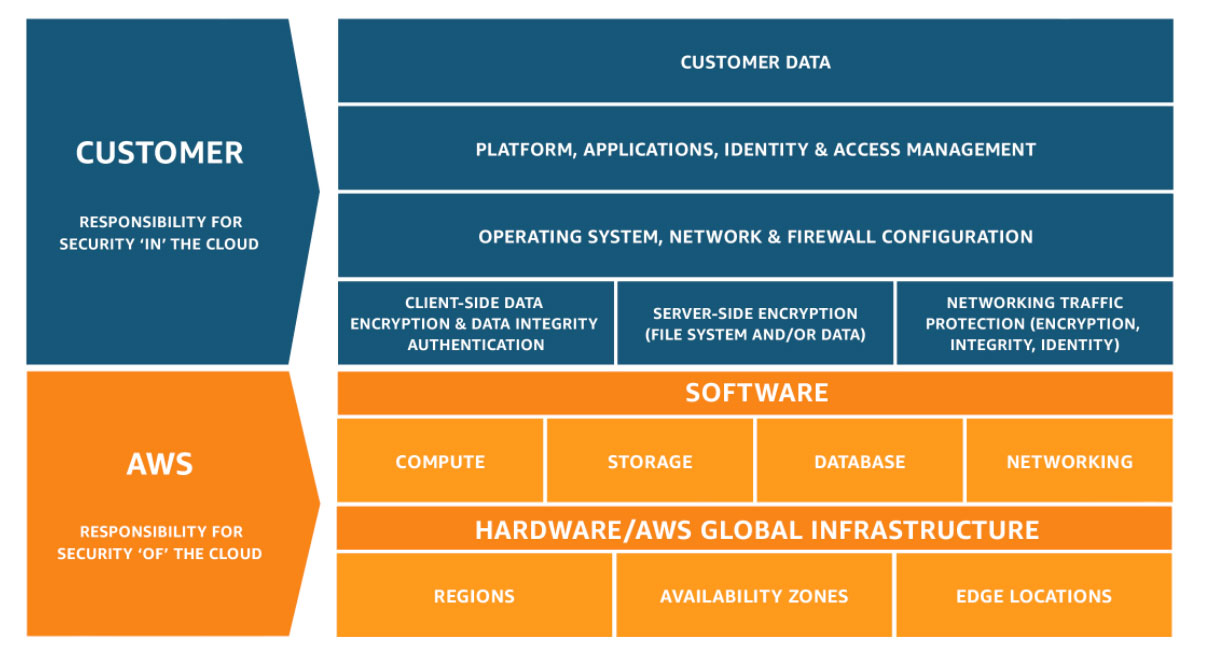
\includegraphics[scale=0.35]{Imagens/modelo_compartilhado_de_responsabilidade.jpg}
    \legend{Fonte: \cite{ref:013}.}
    \label{fig:modelo_compartilhado_de_responsabilidade}
\end{figure}

Além disso, todo tráfego de dados acontece via TLS. TLS é um protocolo criptográfico projetado para fornecer segurança da comunicação em uma rede de computadores. O protocolo é amplamente usado em aplicativos como e-mail e mensagens instantâneas, mas seu uso na proteção de HTTPS continua sendo o mais visível publicamente \cite{ref:014}.

Para o serviço AWS IoT, que será mais bem detalhado na sessão \autoref{section:aws_iot}, cada dispositivo e cliente precisa ter credenciais para a iteração com a rede IoT. O cliente é responsável por gerenciar credencias para cada dispositivo e políticas para o serviço AWS IoT. As credenciais têm o papel de criar identidade única para os dispositivos, enquanto as políticas administram as permissões de cada dispositivo ou grupo de dispositivos.

As credenciais geradas para cada dispositivo são uma forma de autenticação. Autenticação é um mecanismo de verificação de identidade de um cliente e/ou servidor \cite{ref:016}. Um exemplo de certificado é o X.509. Os certificados X.509 são certificados digitais que usam o padrão de infraestrutura de chave pública X.509 para associar uma chave pública a uma identidade contida em um certificado \cite{ref:015}. As cadeias de certificados X.509 são usadas para autenticação de servidor por clientes e autenticação de cliente pelo servidor.

As políticas, por sua vez, são mecanismos de autorização. Autorização é o processo de garantir permissões a uma identidade autenticada \cite{ref:017}. De forma simples, as políticas determinam o que uma identidade autenticada pode fazer. Considere, por exemplo, um dispositivo conectado ao serviço AWS IoT com um certificado X.509. Com um documento de política, esse dispositivo pode ter acesso a todos os tópicos MQTT ou um número restrito de tópicos.

Para o gerenciamento de políticas, a AWS faz uso de documentos no formato JSON. O \autoref{lst:iot_policy} mostra um exemplo de política que dá permissões para um dispositivo IoT acessar recursos do serviço AWS IoT de um usuário raiz com ID 332527922592 e localizado na região ``\textit{sa-east-1}'' (São Paulo).

\begin{lstlisting}[float=htbp,language=json,firstnumber=1,caption={Exemplo de uma política dando permissões de uso do serviço AWS IoT para um dispositivo IoT.},label=lst:iot_policy]
{
    "Effect": "Allow",
    "Action": "iot:Publish",
    "Resource": "arn:aws:iot:sa-east-1:332527922592:*"
},
{
    "Effect": "Allow",
    "Action": "iot:Receive",
    "Resource": "arn:aws:iot:sa-east-1:332527922592:*"
}
\end{lstlisting}

% -----------------------------------------------------------------------------
% Capítulo 2.5 AWS IoT
% -----------------------------------------------------------------------------
\section{AWS IoT}\label{section:aws_iot}

O AWS IoT é um conjunto de serviços em nuvem oferecidos pela AWS que permitem a conexão de dispositivos IoT a outros dispositivos e a outros serviços oferecidos pelo AWS. Em termos simples, o AWS IoT funciona como uma ponte entre dispositivos IoT e os serviços em nuvem que a AWS fornece, assim como pode ser visto na \autoref{fig:what_is_iot}.

\begin{figure}[htbp]
    \centering
    \caption{Integração de dispositivos IoT com serviços AWS por meio do AWS IoT.}
    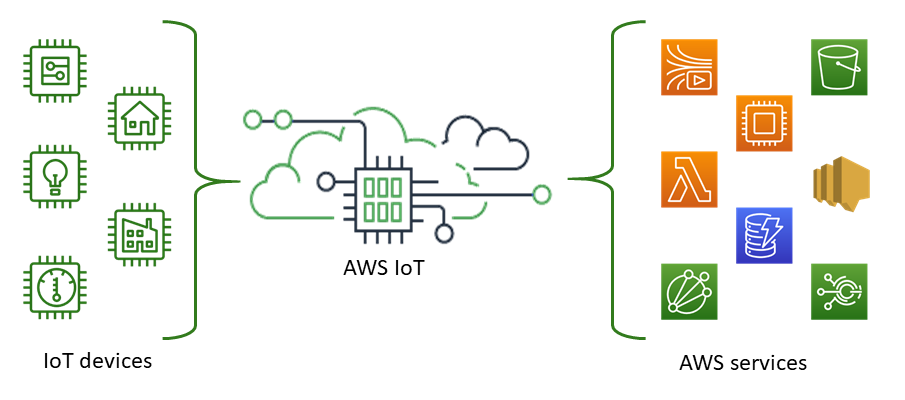
\includegraphics[scale=0.5]{Imagens/what-is-aws-iot.png}
    \legend{Fonte: \cite{ref:018}.}
    \label{fig:what_is_iot}
\end{figure}

Os dispositivos IoT geralmente estão localizados próximos às interfaces do mundo real que monitoram e/ou controlam. Eles geralmente também incluem recursos de computação e armazenamento, como microcontroladores, CPUs e memórias. Alguns exemplos de dispositivos disponíveis no mercado são \cite{ref:019}:

\begin{itemize}
    \item LoRaWAN e dispositivos;
    \item Arduino;
    \item Raspberry PI;
    \item Dispositivos de IoT personalizados.
\end{itemize}

Para a completa integração desses dispositivos com serviços AWS e usuários, alguns componentes são essenciais. Aplicativos de celulares, por exemplo, são utilizados para que o usuário tenha acesso aos seus aparelhos e os configure conforme a sua preferência \cite{ref:019}. Tem-se como outro exemplo os protocolos utilizados para a comunicação dos dispositivos com serviços em nuvem. A tecnologia AWS IoT possui suporte para os seguintes protocolos:

\begin{itemize}
    \item MQTT;
    \item HTTPS;
    \item LoRaWAN.
\end{itemize}

O protocolo MQTT será mais bem detalhado na sessão \autoref{section:mqtt}. Para o desenvolvimento de softwares a nível de dispositivo, o AWS IoT também fornece suporte para um sistema operacional em tempo real para microcontroladores, o FreeRTOS. Alguns exemplos de outros serviços que o AWS IoT oferece suporte podem ser vistos na \autoref{fig:aws_iot_architecture}.

\begin{figure}[htbp]
    \centering
    \caption{Exemplos de serviços fornecidos pelo AWS IoT.}
    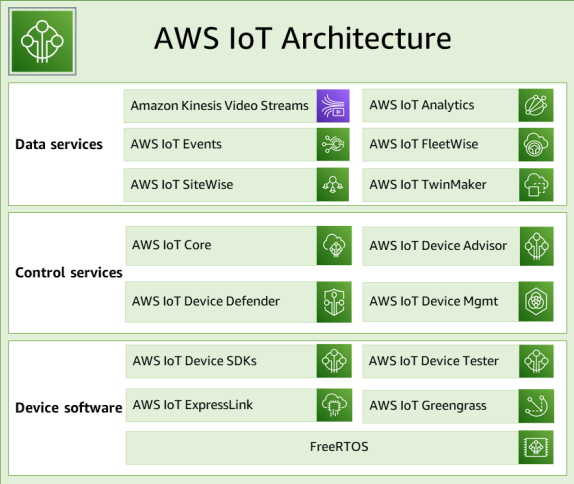
\includegraphics[scale=0.7]{Imagens/aws_iot_architecture.png}
    \legend{Fonte: \cite{ref:019}.}
    \label{fig:aws_iot_architecture}
\end{figure}

O serviço IoT Core será mais bem detalhado na sessão \autoref{subsection:aws_iot_core}.

% ------------------------------------------------------------------------------------------------
% Capítulo 2.5.1 - AWS IoT Core
% -----------------------------------------------------------------------------
\subsection{AWS IoT Core}\label{subsection:aws_iot_core}

O AWS IoT Core é serviço de controle oferecido pela AWS que permite a conexão de bilhões de dispositivos de IoT e rotear trilhões de mensagens para serviços da AWS sem que o usuário tenha que gerenciar a infraestrutura \cite{ref:020}. Esse serviço está disponível gratuitamente para clientes por doze meses a partir da data em que a conta da AWS é criada. Haverá taxas de uso do AWS IoT core após doze meses de uso ou quando a aplicação exceder os níveis de uso gratuito descritos abaixo \cite{ref:021}:

\begin{itemize}
    \item 2.250.000 minutos de conexão;
    \item 500.000 mensagens;
    \item 225.000 operações do Registry ou Device Shadow;
    \item 250.000 regras acionadas e 250.000 ações executadas.
\end{itemize}

Dessa forma, o AWS IoT Core é o serviço que permite a gerência de dispositivos inteligentes. A comunicação do serviço AWS IoT com os nós da rede IoT acontece via protocolo MQTT. Os preços cobrados pela AWS após doze meses de uso ou excedendo os limites já citados pode ser visto abaixo \cite{ref:021}:

\begin{itemize}
    \item Preço da conectividade: 0,12 USD (por milhão de minutos de conexão);
    \item Até 1 bilhão de mensagens MQTT e HTTP: 1,50 USD (por milhão de mensagens);
    \item Próximos 4 bilhões de mensagens MQTT e HTTP: 1,20 USD (por milhão de mensagens);
    \item Mais de 5 bilhões de mensagens MQTT e HTTP: 1,05 USD (por milhão de mensagens).
\end{itemize}

% -----------------------------------------------------------------------------
% Capítulo 2.6 - AWS Lambda
% -----------------------------------------------------------------------------
\section{AWS Lambda}\label{section:aws_lambda}

O AWS Lambda é um serviço que permite a execução de códigos sem que o usuário se preocupe com infraestrutura. A computação ocorre sem servidor e é orientado a eventos \cite{ref:022}. Esses eventos podem ser mudanças de estado ou atualizações, como por exemplo o usuário acionando alguma tarefa através da Alexa. O AWS Lambda permite, também, que o usuário estenda a lógica de outros serviços da AWS. Sumariamente, o serviço AWS Lambda permite que o usuário execute serviços de back-end sem provisionar ou gerenciar servidores.

O nível gratuito do AWS Lambda inclui um milhão de solicitações gratuitas por mês e 400.000 GB-segundos de tempo de computação por mês. Caso esses limites sejam excedidos, a precificação acontece sobre o número total de solicitações feitas por todas as funções. O preço final depende da quantidade de memória alocada por função \cite{ref:023}.

Para começar a usar o AWS Lambda, o usuário deve primeiro carregar o código na nuvem AWS. Isso pode ser feito via AWS CLI, submissão de um arquivo no formato zip ou até mesmo criando o código diretamente no console do Lambda.  O Lambda oferece suporte nativo às linguagens Java, Go, PowerShell, Node.js, C\#, Python e Ruby \cite{ref:024}. Após o carregamento do código, o usuário deve também configurar a memória e o tempo limites da função. Além disso, o usuário deve especificar o recurso que acionará a função. Alguns exemplos de recursos acionadores são uma transmissão do Amazon Kinesis e um evento gerado pela Alexa.

A \autoref{fig:exemplo_aws_lambda} mostra um exemplo de uso do AWS Lambda. Nesse exemplo, a Alexa gera um evento acionador e a função transmite mensagens via tópicos MQTT para o AWS IoT.

\begin{figure}[htbp]
    \centering
    \caption{Exemplos de uso do AWS Lambda com a Alexa gerando um evento acionador.}
    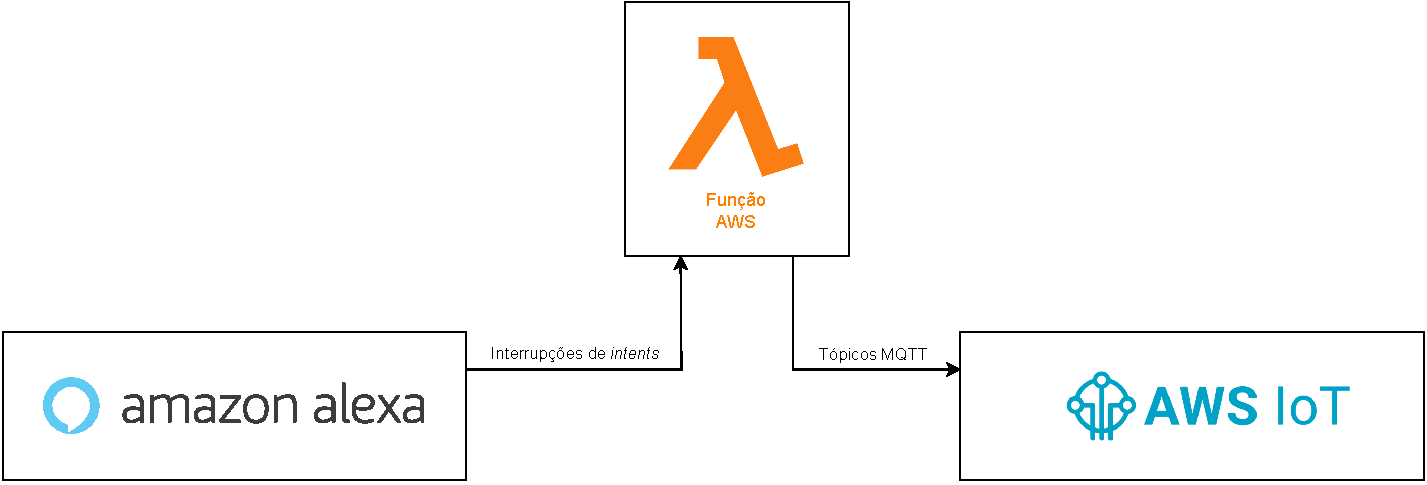
\includegraphics[scale=0.6]{Imagens/exemplo_aws_lambda.pdf}
    \legend{Fonte: Produzido pelo autor (2022).}
    \label{fig:exemplo_aws_lambda}
\end{figure}

% -----------------------------------------------------------------------------
% Capítulo 2.7 - MQTT
% -----------------------------------------------------------------------------
\section{MQTT}\label{section:mqtt}

MQTT é um protocolo de mensagens para dispositivos IoT. Ele foi desenvolvido para dispositivos com limitada disponibilidade de largura de banda (\textit{network bandwidth}). Ele deve ser executado em um protocolo de transporte que forneça conexões bidirecionais ordenadas, sem perdas - normalmente, TCP/IP \cite{ref:025}.

No protocolo MQTT, existem dois tipos de entidades: o \textit{message broker} e os clientes. Um \textit{message broker} é um servidor que tem o papel de receber diversas mensagens dos diversos clientes e, então, as rotear para os clientes de destino. Já um cliente pode ser qualquer dispositivo que se comunica via rede com o \textit{message broker}, a partir de bibliotecas do protocolo MQTT \cite{ref:025}.

As informações são organizadas em hierarquia de tópicos. Quando algum cliente possui um novo item de dados para distribuir, ele envia uma mensagem de controle com os dados para o \textit{message broker}. O \textit{broker}, então, distribui as informações para todos os clientes que se inscreveram nesse tópico. O cliente remetente (\textit{publisher}) não precisa ter nenhuma informação sobre número de clientes que irão receber essa mensagem. Os clientes destinatários, por sua vez, também não precisam ser configurados com nenhuma informação dos destinatários.

Os sete tipos de mensagens existentes no protocolo MQTT são \cite{ref:025}:

\begin{itemize}
    \item \textit{Connect}: Aguarda o estabelecimento de uma conexão com o \textit{message broker} e cria um link entre os nós;
    \item \textit{Disconnect}: Aguarda o fim da tarefa que está sendo executada pelo cliente e desconecta a sessão TCP/IP;
    \item \textit{Publish}: Mensagem a ser distribuída para os clientes inscritos. Mais informações sobre esse tipo de mensagem podem ser encontrado na \autoref{subsection:mqtt_publish_message}.
    \item \textit{Subscribe}: Para receber mensagens sobre tópicos de interesse, o cliente envia uma mensagem \textit{Subscribe} para o \textit{broker}. Mais informações sobre esse tipo de mensagem podem ser encontrado na \autoref{subsection:mqtt_subscribe_message};
    \item \textit{Suback}: Para confirmar cada assinatura, o \textit{broker} envia uma mensagem de confirmação \textit{Suback} ao cliente. Mais informações sobre esse tipo de mensagem podem ser encontrado na \autoref{subsection:mqtt_subscribe_message};
    \item \textit{Unsubscribe}: Esta mensagem exclui as assinaturas existentes de um cliente no \textit{broker}. Mais informações sobre esse tipo de mensagem podem ser encontrado na \autoref{subsection:mqtt_unsubscribe_message};
    \item \textit{Unsuback}: Para confirmar o cancelamento de assinatura, o \textit{broker} envia uma mensagem de confirmação \textit{Unsuback} ao cliente. Mais informações sobre esse tipo de mensagem podem ser encontrado na \autoref{subsection:mqtt_unsuback_message}.
\end{itemize}

Depois que um cliente envia com êxito a mensagem \textit{Subscribe} e recebe a mensagem \textit{Suback}, ele obtém todas as mensagens publicadas de um tópico nas assinaturas contidas da mensagem \textit{Subscribe}. Após receber o \textit{Unsuback} do \textit{broker}, o cliente pode assumir que as assinaturas na mensagem \textit{Unsubscribe} foram excluídas.

Se o \textit{message broker} receber uma mensagem em um tópico para o qual não há assinantes, a mensagem será descartada. Quando um cliente \textit{publisher} se conecta pela primeira vez ao \textit{broker}, ele pode configurar uma mensagem padrão para ser enviada aos assinantes se o \textit{broker} detectar que o cliente \textit{publisher} se desconectou inesperadamente.

Os clientes interagem apenas com um \textit{broker}, mas um sistema pode conter vários \textit{brokers} que trocam informações com base nos tópicos de seus assinantes atuais. Uma mensagem de controle MQTT deve ter entre dois e duzentos e cinquenta e seis bytes. O MQTT conta com o protocolo TCP para transmissão de dados. Uma variante, MQTT-SN, é usada com outros protocolos de transporte, como UDP ou Bluetooth.

A \autoref{fig:rede_mqtt} mostra um exemplo de uma rede MQTT com quatro clientes.

\begin{figure}[htbp]
    \centering
    \caption{Exemplo de uma rede MQTT com quatro clientes.}
    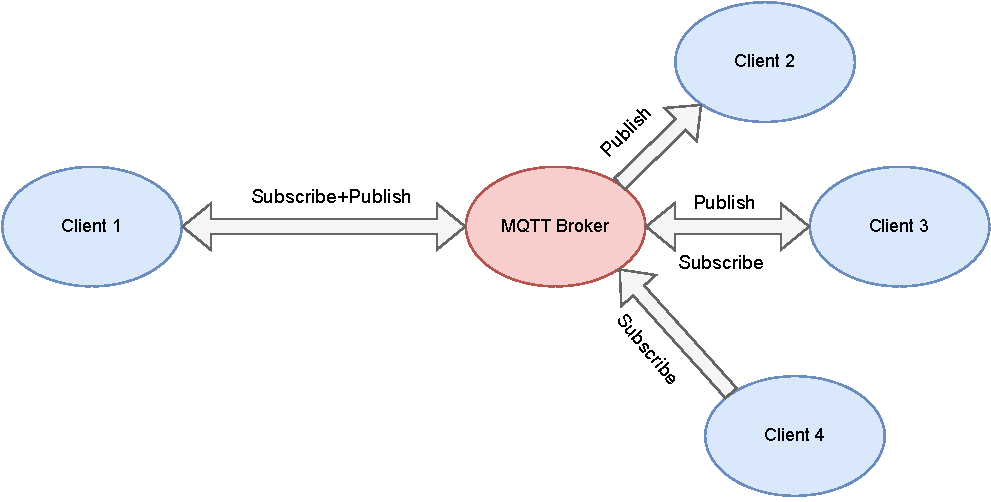
\includegraphics[scale=0.7]{Imagens/mqtt_protocol.pdf}
    \legend{Fonte: Produzido pelo autor (2022).}
    \label{fig:rede_mqtt}
\end{figure}

% -----------------------------------------------------------------------------
% Capítulo 2.5.1 - MQTT Publish Message
% -----------------------------------------------------------------------------
\subsection{MQTT Publish Message}\label{subsection:mqtt_publish_message}

O formato de uma mensagem do tipo \textit{Publish} está apresentado na \autoref{fig:mqtt_publish_message_attributes}.

\begin{figure}[htbp]
    \centering
    \caption{Atributos de uma mensagem do tipo \textit{Publish} para o protocolo MQTT.}
    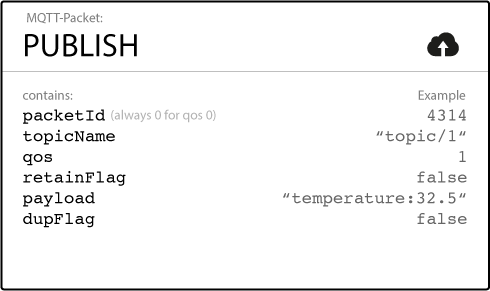
\includegraphics[scale=0.5]{Imagens/mqtt_publish_message_attributes.png}
    \legend{Fonte: \cite{ref:026}.}
    \label{fig:mqtt_publish_message_attributes}
\end{figure}

Os atributos de uma mensagem do tipo \textit{Publish} são caracterizados abaixo \cite{ref:026}:

\begin{itemize}
    \item packetId: O identificador de pacote identifica exclusivamente uma mensagem;
    \item topicName: O nome do tópico é uma \textit{string} simples que é estruturada hierarquicamente com barras como delimitadores (``alexa/builtin/device'', por exemplo);
    \item qos: Indica o nível de qualidade de serviço (QoS) da mensagem. Existem três níveis: 0, 1 e 2. O nível de serviço determina que tipo de garantia uma mensagem tem para chegar ao destinatário pretendido (cliente ou \textit{broker}).
    \item retainFlag: Sinalizador indicando se a mensagem é salva pelo \textit{broker} como o último valor válido conhecido para um tópico especificado. Quando um novo cliente se inscreve em um tópico, ele recebe a última mensagem retida nesse tópico.
    \item payLoad: Conteúdo da mensagem. O MQTT é \textit{data-agnostic}. Ou seja, é possível enviar qualquer tipo de informação que pode ser codificada em formato binário.
    \item dupFlag: Indica se a mensagem é uma duplicata e foi reenviada porque o destinatário pretendido (cliente ou \textit{broker}) não enviou uma resposta de \textit{acknowledge}.
\end{itemize}

% -----------------------------------------------------------------------------
% Capítulo 2.5.2 - MQTT Subscribe Message
% -----------------------------------------------------------------------------
\subsection{MQTT Subscribe Message}\label{subsection:mqtt_subscribe_message}

O formato de uma mensagem do tipo \textit{Subscribe} está apresentado na \autoref{fig:mqtt_subscribe_message_attributes}. Esta mensagem de assinatura é muito simples, contém um identificador de pacote exclusivo e uma lista de assinaturas.

\begin{figure}[htbp]
    \centering
    \caption{Atributos de uma mensagem do tipo \textit{Subscribe} para o protocolo MQTT.}
    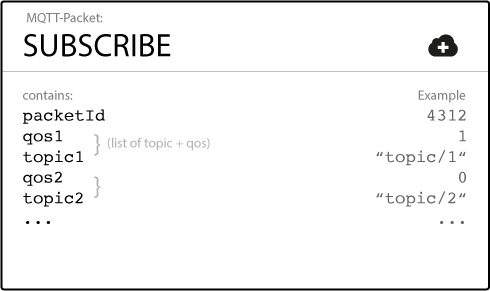
\includegraphics[scale=0.5]{Imagens/mqtt_subscribe_message_attributes.png}
    \legend{Fonte: \cite{ref:026}.}
    \label{fig:mqtt_subscribe_message_attributes}
\end{figure}

Os atributos de uma mensagem do tipo \textit{Subscribe} são caracterizados abaixo \cite{ref:026}:

\begin{itemize}
    \item packetId: O identificador de pacote identifica exclusivamente uma mensagem;
    \item \textit{List of Subscriptions}: Uma mensagem \textit{Subscribe} pode conter várias assinaturas para um cliente. Cada assinatura é composta por um tópico (\textit{topici}) e um nível de QoS (\textit{qosi}). O tópico pode conter \textit{wildcards} que possibilitam a assinatura de um padrão de tópicos em vez de um tópico específico. Se houver assinaturas sobrepostas para um cliente, o \textit{broker} entrega a mensagem que possui o nível de QoS mais alto para esse tópico.
\end{itemize}

% -----------------------------------------------------------------------------
% Capítulo 2.5.3 - MQTT Suback Message
% -----------------------------------------------------------------------------
\subsection{MQTT Suback Message}\label{subsection:mqtt_suback_message}

O formato de uma mensagem do tipo \textit{Suback} está apresentado na \autoref{fig:mqtt_suback_message_attributes}. Esta mensagem contém o identificador de pacote da mensagem \textit{Subscribe} original e uma lista de códigos de retorno.

\begin{figure}[htbp]
    \centering
    \caption{Atributos de uma mensagem do tipo \textit{Suback} para o protocolo MQTT.}
    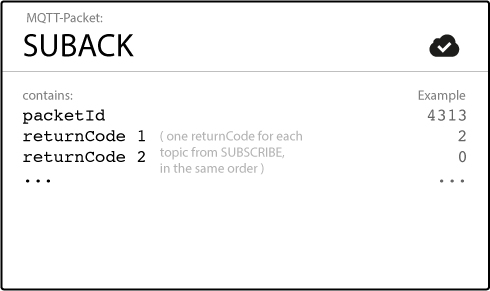
\includegraphics[scale=0.5]{Imagens/mqtt_suback_message_attributes.png}
    \legend{Fonte: \cite{ref:026}.}
    \label{fig:mqtt_suback_message_attributes}
\end{figure}

Os atributos de uma mensagem do tipo \textit{Suback} são caracterizados abaixo \cite{ref:026}:

\begin{itemize}
    \item packetId: O identificador de pacote identifica exclusivamente uma mensagem;
    \item \textit{Return Code}: O \textit{broker} envia um código de retorno para cada par de tópico/QoS que recebe de mensagens \textit{Subscribe}. O código de retorno reconhece cada tópico e mostra o nível de QoS concedido pelo \textit{broker}. Se o \textit{broker} recusar uma assinatura, a mensagem \textit{Suback} conterá um código de retorno de falha para esse tópico específico.
\end{itemize}

% -----------------------------------------------------------------------------
% Capítulo 2.5.4 - MQTT Unsubscribe Message
% -----------------------------------------------------------------------------
\subsection{MQTT Unsubscribe Message}\label{subsection:mqtt_unsubscribe_message}

O formato de uma mensagem do tipo \textit{Unsubscribe} está apresentado na \autoref{fig:mqtt_unsubscribe_message_attributes}. A mensagem \textit{Unsubscribe} é semelhante à mensagem  \textit{Subscribe} e possui um identificador de pacote e uma lista de tópicos.

\begin{figure}[htbp]
    \centering
    \caption{Atributos de uma mensagem do tipo \textit{Unsubscribe} para o protocolo MQTT.}
    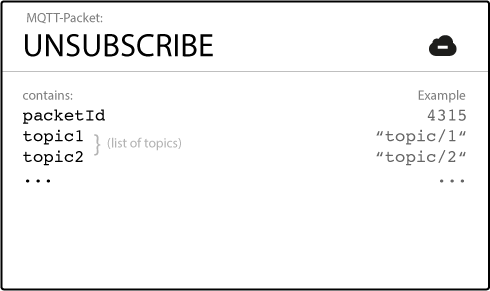
\includegraphics[scale=0.5]{Imagens/mqtt_unsubscribe_message_attributes.png}
    \legend{Fonte: \cite{ref:026}.}
    \label{fig:mqtt_unsubscribe_message_attributes}
\end{figure}

Os atributos de uma mensagem do tipo \textit{Unsubscribe} são caracterizados abaixo \cite{ref:026}:

\begin{itemize}
    \item packetId: O identificador de pacote identifica exclusivamente uma mensagem;
    \item \textit{List of Topic}: A lista de tópicos pode conter vários tópicos dos quais o cliente deseja cancelar a assinatura. Só é necessário enviar o tópico (sem QoS). O \textit{broker} cancela a assinatura do tópico, independentemente do nível de QoS com o qual foi originalmente assinado.
\end{itemize}

% -----------------------------------------------------------------------------
% Capítulo 2.5.5 - MQTT Unsuback Message
% -----------------------------------------------------------------------------
\subsection{MQTT Unsuback Message}\label{subsection:mqtt_unsuback_message}

O formato de uma mensagem do tipo \textit{Unsuback} está apresentado na \autoref{fig:mqtt_unsuback_message_attributes}. Esta mensagem contém apenas o identificador de pacote da mensagem \textit{Unsubscribe} original.

\begin{figure}[htbp]
    \centering
    \caption{Atributos de uma mensagem do tipo \textit{Unsuback} para o protocolo MQTT.}
    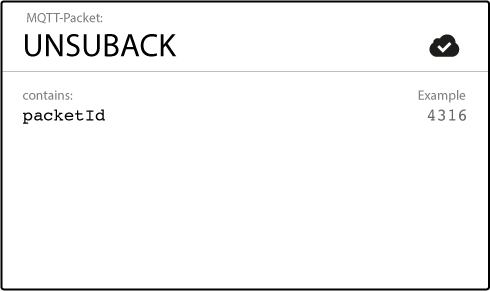
\includegraphics[scale=0.5]{Imagens/mqtt_unsuback_message_attributes.png}
    \legend{Fonte: \cite{ref:026}.}
    \label{fig:mqtt_unsuback_message_attributes}
\end{figure}

% -----------------------------------------------------------------------------
% Capítulo 2.6 - Amazon Alexa
% -----------------------------------------------------------------------------
\section{Amazon Alexa}\label{section:amazon_alexa}

A Amazon Alexa, conhecida simplesmente como Alexa, é uma assistente virtual inteligente capaz de controlar dispositivos inteligentes e ter iterações de voz com os usuários. As capacidades da Alexa podem ser expandidas por terceiros através da instalação de habilidades (aplicativos). Algumas categorias de habilidades em destaque são: Notícias, Negócios e Finanças, Jogos e Curiosidades, Saúde e Boa Forma e Produtividade \cite{ref:002}. A loja oficial de habilidades da Amazon permite que o usuário faça busca de habilidades por categorias, assim como pode ser visto na \autoref{fig:alexa_skills_categorias}.

\begin{figure}[htbp]
    \centering
    \caption{Busca de habilidades da Alexa por categorias.}
    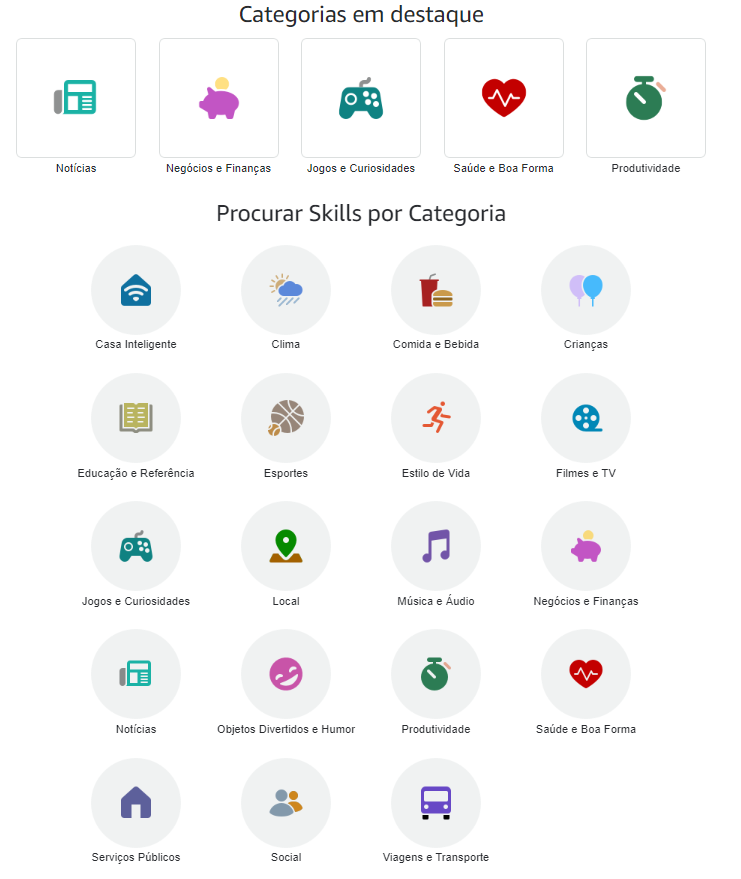
\includegraphics[scale=0.8]{Imagens/alexa_skills_categorias.png}
    \legend{Fonte: \cite{ref:028}.}
    \label{fig:alexa_skills_categorias}
\end{figure}

\subsection{Alexa Skills Kit}\label{subsection:alexa_skills_kit}
O ASK fornece APIs e ferramentas para a criação de habilidades Alexa. Empresas podem desenvolver habilidades para seus produtos e serviços, ou contratarem uma agência especialista em Alexa. Uma habilidade Alexa tem tanto uma interface de voz com o usuário, como uma lógica de aplicativo \cite{ref:029}.

Quando um usuário interage com um dispositivo Alexa, ocorre um processamento da fala no contexto do seu modelo de interação para interpretar o que foi requisitado. A Alexa, então, envia a solicitação à sua lógica de aplicação, responsável por processar e computar essa informação \cite{ref:029}. Essa computação acontece em nuvem AWS ou outro servidor. Dessa forma, caracteriza-se o processamento da fala e interpretação do que foi requisitado como front-end e a computação da lógica de aplicação como back-end. A \autoref{fig:diagrama_habilidades_alexa} mostra um diagrama produzido pela Amazon explicando o funcionamento de uma habilidade Alexa.

\begin{figure}[htbp]
    \centering
    \caption{Diagrama explicando o funcionamento de uma habilidade Alexa.}
    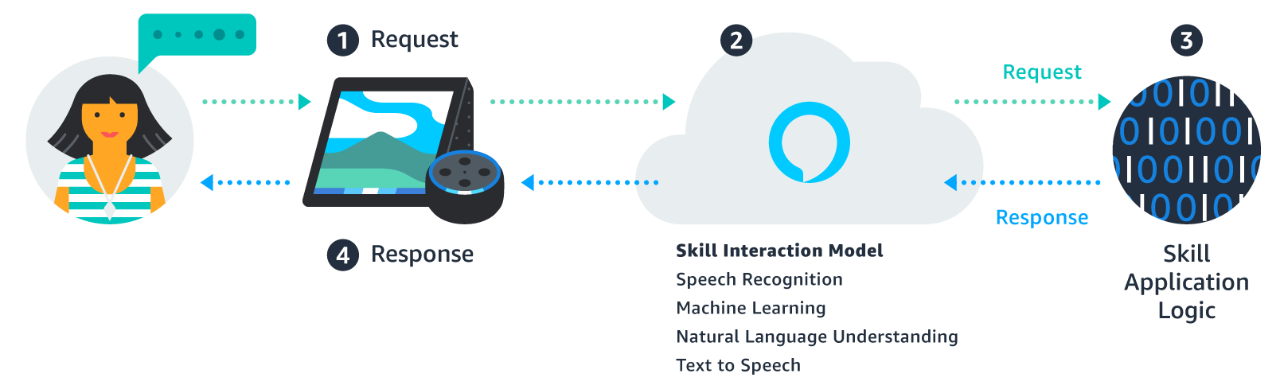
\includegraphics[scale=0.35]{Imagens/diagrama_habilidades_alexa.png}
    \legend{Fonte: \cite{ref:029}.}
    \label{fig:diagrama_habilidades_alexa}
\end{figure}

Para o desenvolvimento de software, os ASK SDKs permitem uma redução da complexidade do projeto. Os SDKs para Java, Node.js e Python fornecem funções específicas da linguagem para tarefas comuns, permitindo a concentração na lógica das habilidades, não no código padrão \cite{ref:029}. A Amazon também fornece distintas de ferramentas de desenvolvimento. O desenvolvedor pode usar o console do portal ou CLI do ASK para criar, gerenciar, testar e publicar habilidades.

\subsection{Alexa Voice Service}\label{subsection:alexa_voice_service}

A Amazon permite que fabricantes construam dispositivos com a Alexa integrada usando o AVS, um serviço baseado na AWS com APIs que permitem a integração de dispositivos com a Alexa. Dessa forma, produtos usuários do AVS têm acesso a diversos recursos da Alexa, incluindo as habilidades Alexa. A principal vantagem do AVS é o fornecimento de APIs que permitem o reconhecimento automático de fala, com computação executada em nuvem, e compreensão de linguagem natural \cite{ref:002}.

Um exemplo de uso do AVS é um dispositivo IoT com a Alexa embutida. Nesse exemplo, o desenvolvedor fará uso dos serviços AVS, AWS IoT e Login da Amazon. Um diagrama desenvolvido pela Amazon mostrando um exemplo de integração do AVS ao AWS IoT pode ser visto na \autoref{fig:integracao_avs_aws_iot}.

\begin{figure}[htbp]
    \centering
    \caption{Diagrama de integração do AVS ao serviço AWS IoT Core.}
    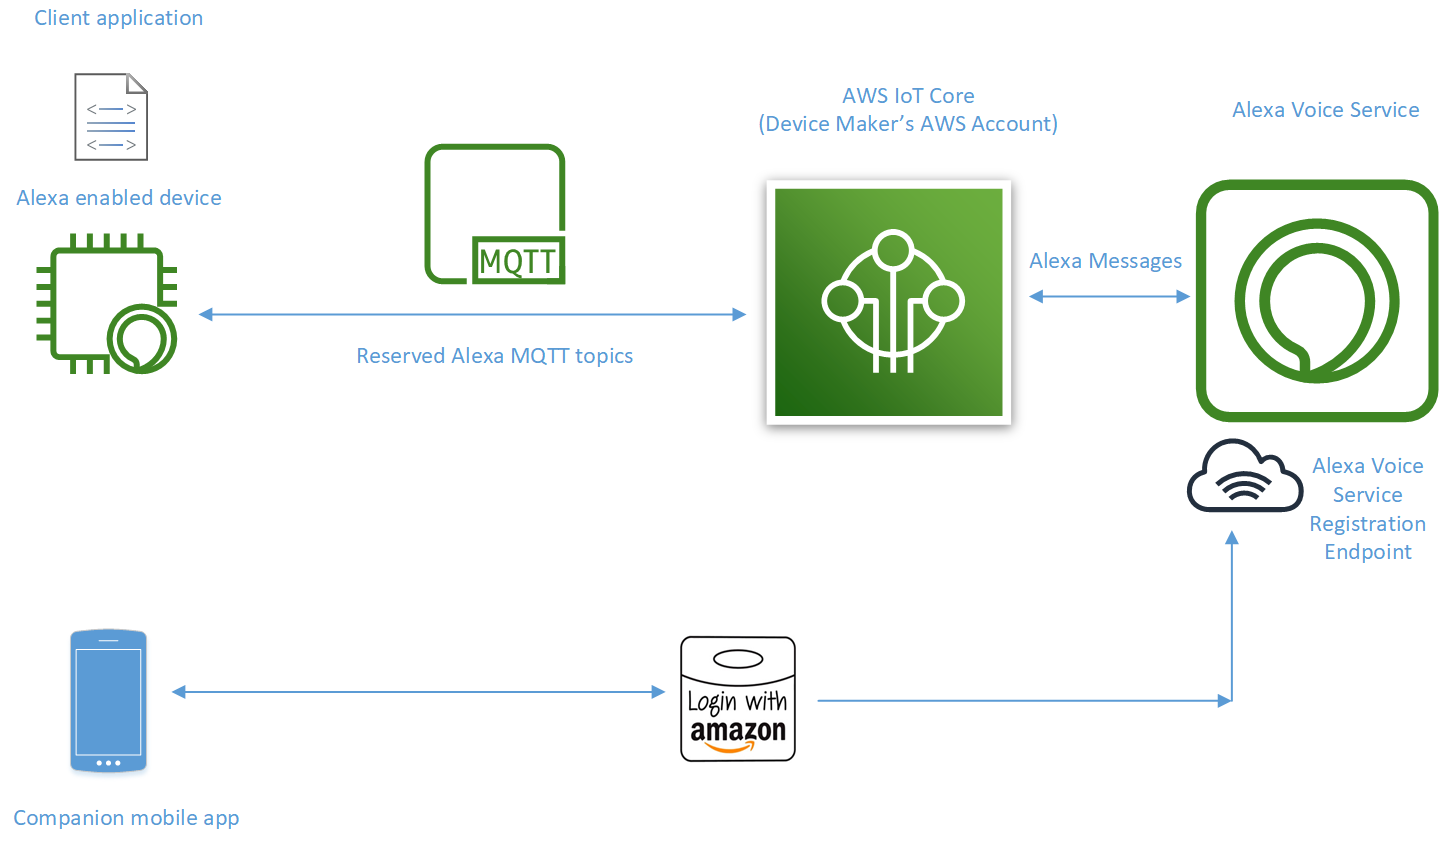
\includegraphics[scale=0.6]{Imagens/integracao_avs_aws_iot.png}
    \legend{Fonte: \cite{ref:030}.}
    \label{fig:integracao_avs_aws_iot}
\end{figure}

% -----------------------------------------------------------------------------
% Capítulo 2.6 - Trabalhos Correlatos
% -----------------------------------------------------------------------------
\section{Trabalhos correlatos}

Essa sessão busca detalhar dois trabalhos correlatos ao protótipo desse trabalho. Os dois trabalhos escolhidos são:

\begin{itemize}
    \item PROTÓTIPO DE AUTOMAÇÃO RESIDENCIAL UTILIZANDO UMA ASSISTENTE DE VOZ, de Leandro Dallarosa Neto;
    \item \textit{Creating an Alexa voice controlled IoT using a Raspberry Pi}, de John Allwork;
\end{itemize}

% -----------------------------------------------------------------------------
% Capítulo 2.6.1 - PROTÓTIPO DE AUTOMAÇÃO RESIDENCIAL UTILIZANDO UMA ASSISTENTE DE VOZ
% -----------------------------------------------------------------------------
\subsection{PROTÓTIPO DE AUTOMAÇÃO RESIDENCIAL UTILIZANDO UMA ASSISTENTE DE VOZ}\label{subsection:prototipo_de_automacao_residencial_utilizando_uma_assistente_de_voz}

Esse projeto foi desenvolvido como um Trabalho de Conclusão de Curso do aluno Leandro Dallarosa Neto, pela Universidade Regional de Blumenau \cite{ref:031}. Em resumo, o projeto teve como escopo a criação de um protótipo de automação residencial por comandos de voz utilizando a assistente pessoal Alexa. O protótipo desenvolvido utilizava o microcontrolador Arduino Ameba para controlar luzes, abrir uma porta magnética e enviar dados de temperatura para o servidor HTTP Thingspeak (2018). A computação do projeto foi feita via serviços em nuvem da AWS: o AWS Iot e o AWS Lambda. A execução do protótipo acontece por comandos de voz recebidos em um aplicativo de dispositivos móveis.

Para testes com o protótipo, uma maquete e um circuito foram montado. Esse circuito conta com o microcontrolador Arduino Ameba, dois módulos relé para Arduino, um regulador de tensão, um eletroímã de 12V e o sensor de temperatura DHT11. A \autoref{fig:circuito_eletronico_leandro_dallarosa} mostra o circuito eletrônico completo da maquete, enquanto a \autoref{fig:maquete_leandro_dallarosa} mostra a vista frontal da maquete.

\begin{figure}[htbp]
    \centering
    \caption{Circuito eletrônico completo da maquete do projeto ``PROTÓTIPO DE AUTOMAÇÃO RESIDENCIAL UTILIZANDO UMA ASSISTENTE DE VOZ''.}
    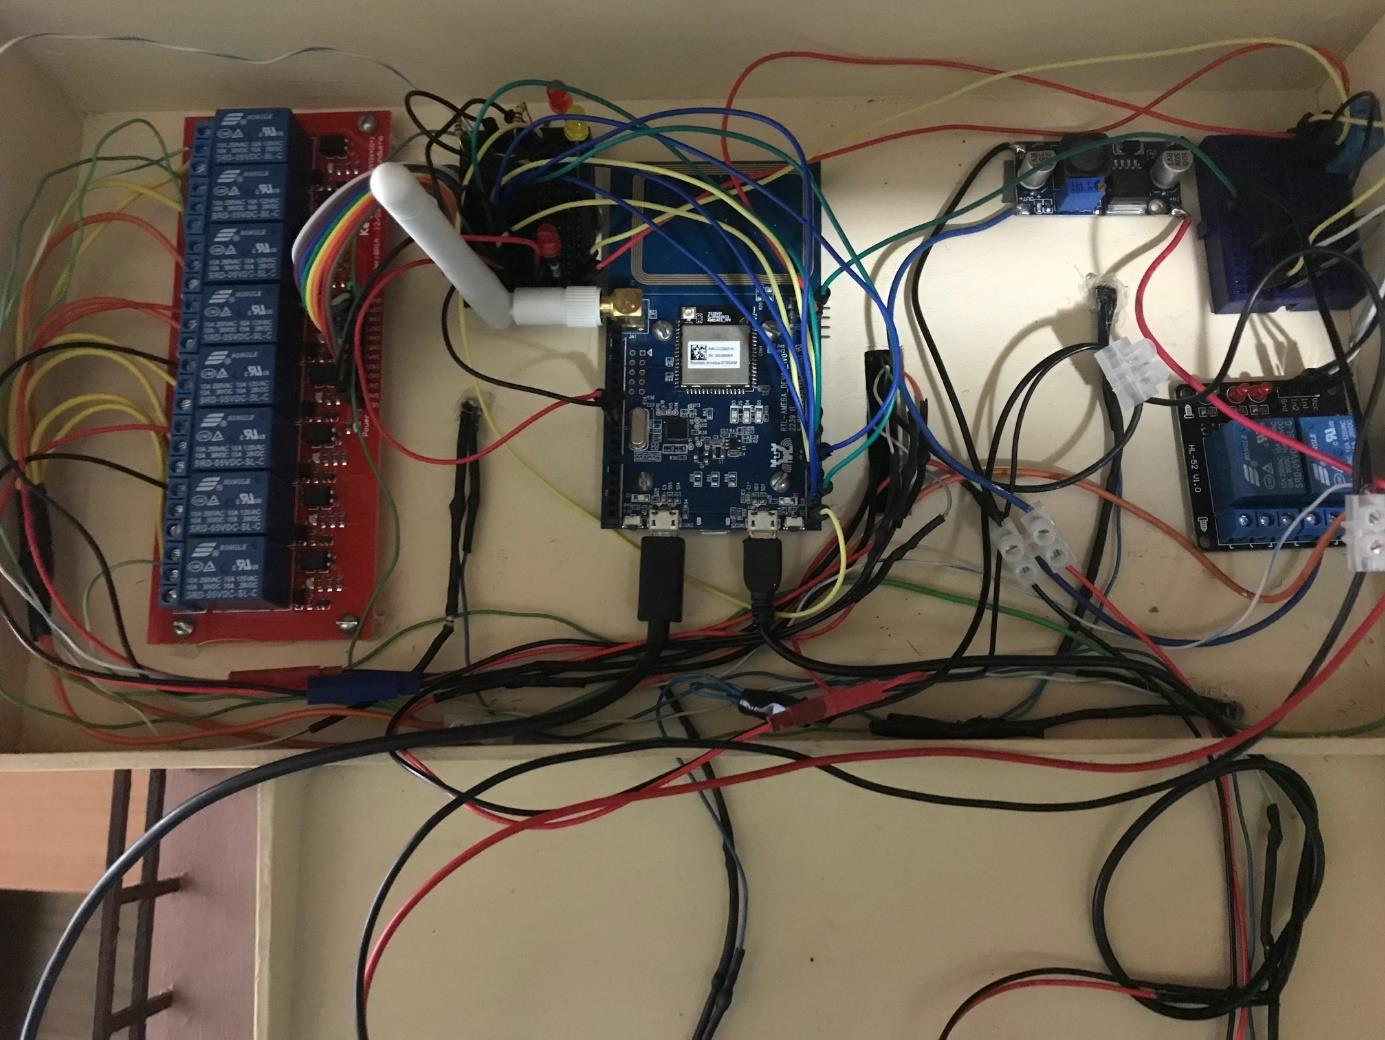
\includegraphics[scale=0.4]{Imagens/circuito_eletronico_leandro_dallarosa.png}
    \legend{Fonte: \cite{ref:031}.}
    \label{fig:circuito_eletronico_leandro_dallarosa}
\end{figure}

\begin{figure}[htbp]
    \centering
    \caption{Imagem frontal da maquete do projeto ``PROTÓTIPO DE AUTOMAÇÃO RESIDENCIAL UTILIZANDO UMA ASSISTENTE DE VOZ''.}
    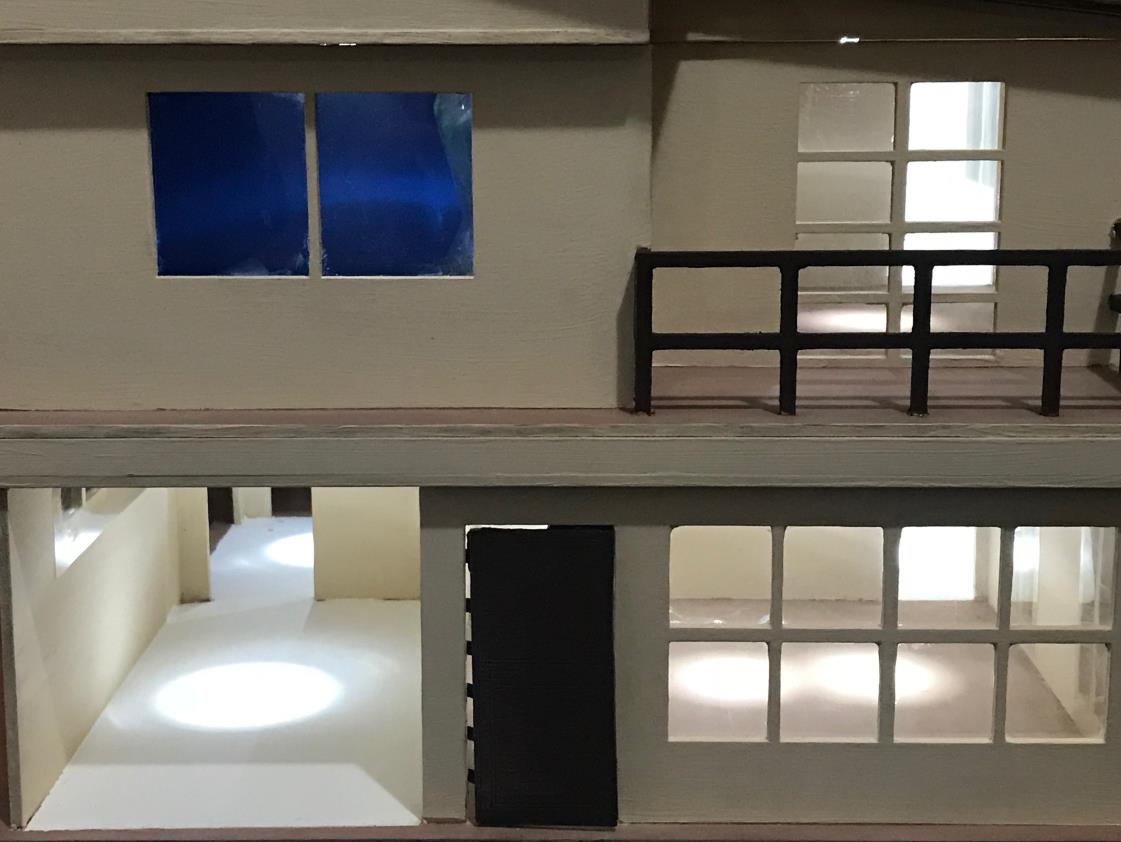
\includegraphics[scale=0.4]{Imagens/maquete_leandro_dallarosa.png}
    \legend{Fonte: \cite{ref:031}.}
    \label{fig:maquete_leandro_dallarosa}
\end{figure}

% -----------------------------------------------------------------------------
% Capítulo 2.6.2 - PROTÓTIPO DE AUTOMAÇÃO RESIDENCIAL UTILIZANDO UMA ASSISTENTE DE VOZ
% -----------------------------------------------------------------------------
\subsection{\textit{Creating an Alexa voice controlled IoT using a Raspberry Pi}}\label{subsection:creating_an_alexa_voice_controlled_iot_using_a_raspberry_pi}

Esse projeto foi desenvolvido em 2019 pelo YouTuber John Allwork com o objetivo de demonstrar um Raspberry Pi sendo controlado por voz através da Alexa \cite{ref:032}. O projeto conta com uma sequência de vídeos e documentação textual de como criar o seu nó IoT na rede AWS, carregar o código exemplo no AWS Lambda, criar habilidades na Alexa developer console e carregar o \textit{firmware} em um Raspberry Pi 4.

A \autoref{fig:testing_our_raspberrypi_thing} mostra uma captura de tela do vídeo 5 da sequência de vídeos do projeto do YouTuber John Allwork.

\begin{figure}[htbp]
    \centering
    \caption{Captura de tela do vídeo 5 da sequência de vídeos do projeto ``\textit{Creating an Alexa voice controlled IoT using a Raspberry Pi}''.}
    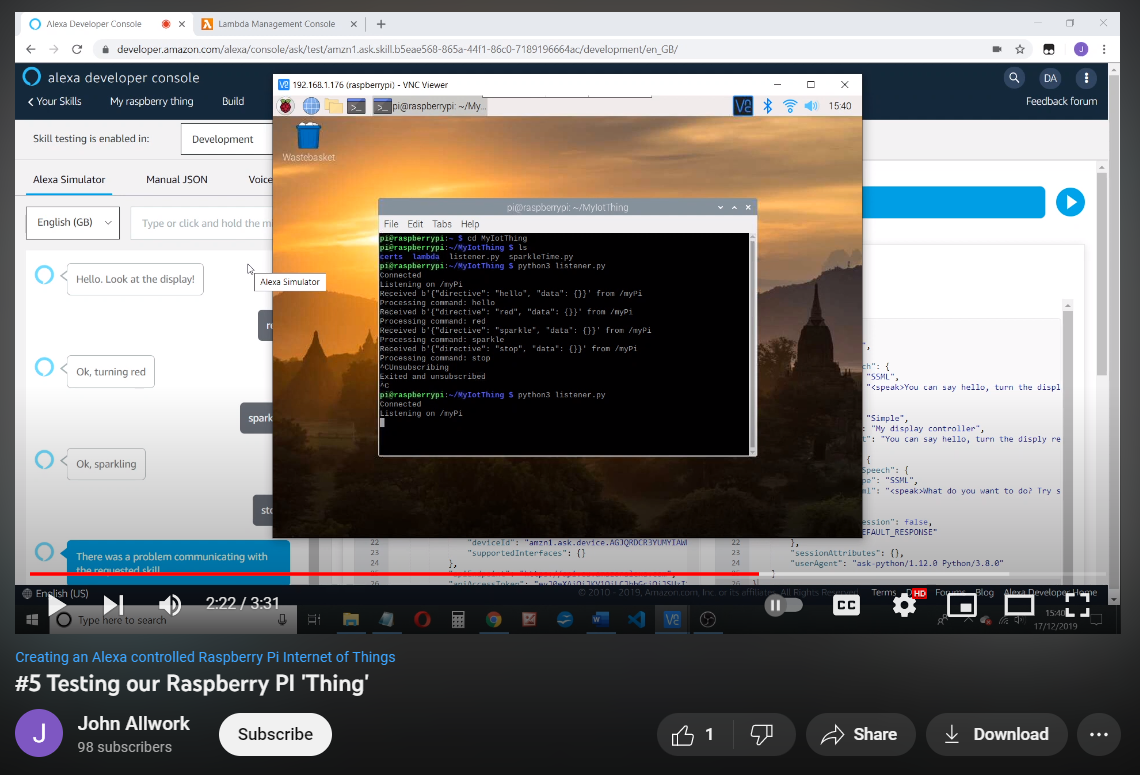
\includegraphics[scale=0.75]{Imagens/testing_our_raspberrypi_thing.png}
    \legend{Fonte: Produzido pelo autor (2022).}
    \label{fig:testing_our_raspberrypi_thing}
\end{figure}


% -----------------------------------------------------------------------------
% Capítulo 3 - Metodologia
% -----------------------------------------------------------------------------
\chapter{Metodologia}\label{chapter:metodologia}

% -----------------------------------------------------------------------------
% Capítulo 3.1 - Objetivos
% -----------------------------------------------------------------------------
\section{Objetivos}

Em resumo, o projeto propõe um protótipo de um nó IoT acionado pela Alexa. O protótipo comunicará com o serviço AWS IoT via tópicos MQTT - protocolo também utilizado na integração do AWS IoT com a Alexa. A \autoref{fig:project_diagram} mostra um diagrama em alto nível do projeto.

\begin{figure}[htbp]
    \centering
    \caption{Diagrama em alto nível do protótipo acionado pela Alexa e integrado ao serviço AWS IoT.}
    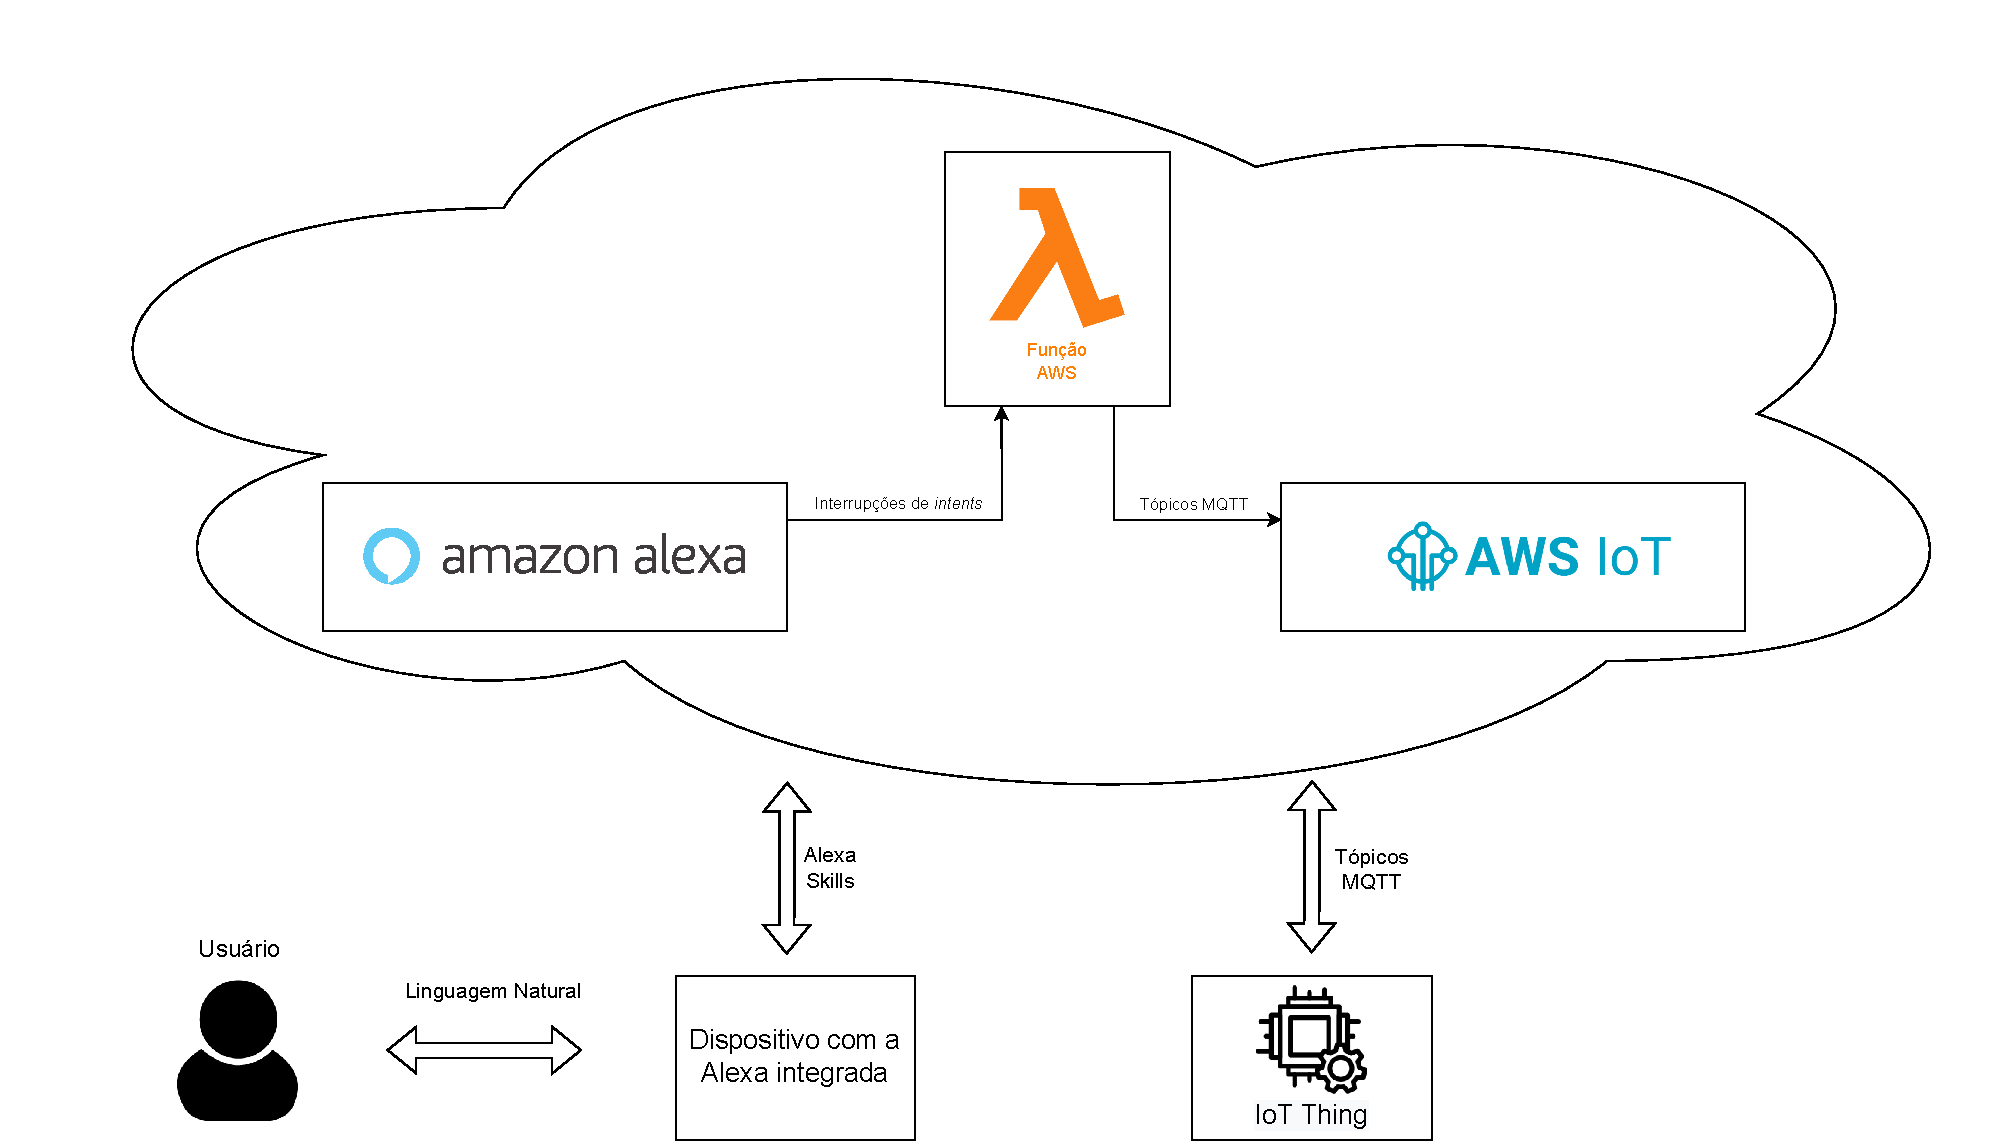
\includegraphics[scale=0.47]{Imagens/project_diagram.pdf}
    \legend{Fonte: Produzido pelo autor (2022).}
    \label{fig:project_diagram}
\end{figure}

Para esse dispositivo, tem-se os seguintes requisitos funcionais:

\begin{alineas}
    \item Suporte à rede Wifi IEEE 802.11 (2,4 GHz);
    \item Possibilidade de se comportar como um nó IoT;
    \item Suporte ao protocolo MQTT;
    \item Possibilidade de comunicação do usuário com o dispositivo em linguagem natural, a partir de microfones;
    \item Possibilidade de implementação de uma Alexa integrada;
    \item Possibilidade de acionamento da Alexa por voz ou toque;
    \item Microfones capazes de entender o usuário em ambientes ruidosos;
\end{alineas}

A seguir, tem-se os requisitos não-funcionais:

\begin{alineas}
    \item Ser um dispositivo qualificado pela AWS;
    \item Baixo custo de prototipagem;
    \item Versatilidade;
\end{alineas}

% -----------------------------------------------------------------------------
% Capítulo 3.2 - Projeto de Hardware
% -----------------------------------------------------------------------------
\section{Projeto de Hardware}

Uma vez escolhidos os requisitos funcionais e não-funcionais do projeto, inicia-se o projeto de hardware. Tomando o baixo custo de prototipagem como um importante requisito do projeto, optou-se pelo uso de sistemas embarcados no projeto. Computadores e notebooks pessoais, por exemplo, possuem um propósito geral e um alto valor agregado, enquanto um sistema embarcado realiza um conjunto de tarefas predefinidas e normalmente possuem um menor valor agregado (PrimeUP, 2022). Isso posto, inicia-se o estudo dos requisitos de um hardware a ser utilizado em aplicações IoT. Como um dos requisitos funcionais é a possibilidade de implementação de uma Alexa integrada, estuda-se os parâmetros mínimos recomendados pela AWS para um dispositivo com a Alexa integrada. Esses requisitos podem ser vistos na \autoref{table:reduced_hardware_footprint}.

% TODO: Converter a tabela para o formato ABNT!
% \begin{longtable}[]{@{}cccc@{}}
% 	\caption{Demonstration of simple table syntax.}\tabularnewline
% 	% \toprule
% 	% Right & Left & Center & Default\tabularnewline
% 	% \midrule
% 	% \endfirsthead
% 	\toprule
% 	Right & Left & Center & Default\tabularnewline
% 	\midrule
% 	\endhead
% 	12    & 12   & 12     & 12\tabularnewline
% 	123   & 123  & 123    & 123\tabularnewline
% 	1     & 1    & 1      & 1\tabularnewline
% 	\bottomrule
% 	\caption*{Fonte: Autor.}
% 	\label{mytable}
% \end{longtable}

% \begin{longtable}[]{@{}cccccc@{}}
% 	\caption{Demonstration of simple table syntax.}\tabularnewline
% 	\toprule
% 	Processador & RAM & SO & Conectividade & \# de Microfones & Alto-falante\tabularnewline
% 	\midrule
% 	\endfirsthead
% 	\toprule
% 	Processador & RAM & SO & Conectividade & \# de Microfones & Alto-falante\tabularnewline
% 	\midrule
% 	\endhead
% 	\begin{tabular}[c]{@{}c@{}}ARM M7 or equivalent\\ Arm M4 + AFE DSP\end{tabular} & \begin{tabular}[c]{@{}c@{}}MB for ARM M7\\ 500KB for M4 + AFE DSP\end{tabular} & FreeRTOS & MQTT/Wi-Fi & 2+ & Otimizado para reprodução de fala \\hline
% 	\bottomrule
% 	\caption*{Fonte: Autor.}
% 	\label{mytable}
% \end{longtable}

\begin{table}[htbp]
    \centering
    \begin{tabular}{|c|c|}
        \hline
        \textbf{Processador}      & \begin{tabular}[c]{@{}c@{}}ARM M7 or equivalent\\ Arm M4 + AFE DSP\end{tabular} \\ \hline
        \textbf{RAM}              & \begin{tabular}[c]{@{}c@{}}MB for ARM M7\\ 500KB for M4 + AFE DSP\end{tabular}  \\ \hline
        \textbf{Target OS}        & FreeRTOS                                                                        \\ \hline
        \textbf{Conectividade}    & MQTT/Wi-Fi                                                                 \\ \hline
        \textbf{\# de Microfones} & 2+                                                                              \\ \hline
        \textbf{Alto-falante}     & Optimized for speech playback                                                   \\ \hline
    \end{tabular}
    \caption{Parâmetros mínimos recomendados pela AWS para o desenvolvimento de um dispositivo de IoT integrado à AVS.}
    \label{table:reduced_hardware_footprint}
\end{table}

Para a prototipagem, alguns kits de desenvolvimento disponíveis no mercado foram estudados. As tabelas \autoref{table:development_kit_a} e \autoref{table:development_kit_b}, presentes no \autoref{chapter:apendice}, mostram informações coletadas de cinco diferentes kits.

Assim como pode ser visto na \autoref{table:reduced_hardware_footprint}, A AWS recomenda o Sistema Operacional FreeRTOS, descartando o \textit{CORE-V MCU DevKit}. Ademais, definiu-se como requisito funcional a possibilidade de comunicação do usuário com o dispositivo através de linguagem natural, demandando no mínimo dois microfones e descartando o \textit{Home Hub 100 Dev Kit for Amazon AVS}.

Por fim, restando somente os dispositivos \textit{STEVAL-VOICE-UI}, \textit{B-L475E-IOT01A2} e \textit{SLN-ALEXA-IOT}, avaliou-se o preço nas lojas oficiais. Os preços, em Novembro de 2022, são respectivamente: \$248.75, \$51,94 e \$171,35. Essa discrepância de valores acontece devido à diferença nas especificações: o segundo dispositivo possui processador Arm® Cortex®-M4, enquanto o primeiro e o terceiro processadores Arm® Cortex®-M7 e Dual Arm® Cortex®-A7, respectivamente. Outrossim, os dispositivos \textit{STEVAL-VOICE-UI} e \textit{SLN-ALEXA-IOT} também contam com alto-falantes, já o \textit{B-L475E-IOT01A2} não. Vale lembrar que a possibilidade de comunicação do dispositivo com o usuário via alto-falante não é um requisito funcional do projeto.

Dessa forma, conclui-se que o kit \textit{B-L475E-IOT01A2} é o dispositivo, com menor custo, que mais se aproxima dos requisitos mínimos especificados pela AWS e atende os requisitos funcionais do projeto. O kit escolhido por ser visto na \autoref{fig:B-L475E-IOT01A2}.

\begin{figure}[htbp]
    \centering
    \caption{Kit de desenvolvimento escolhido para ser protótipo do projeto (\textit{B-L475E-IOT01A2}).}
    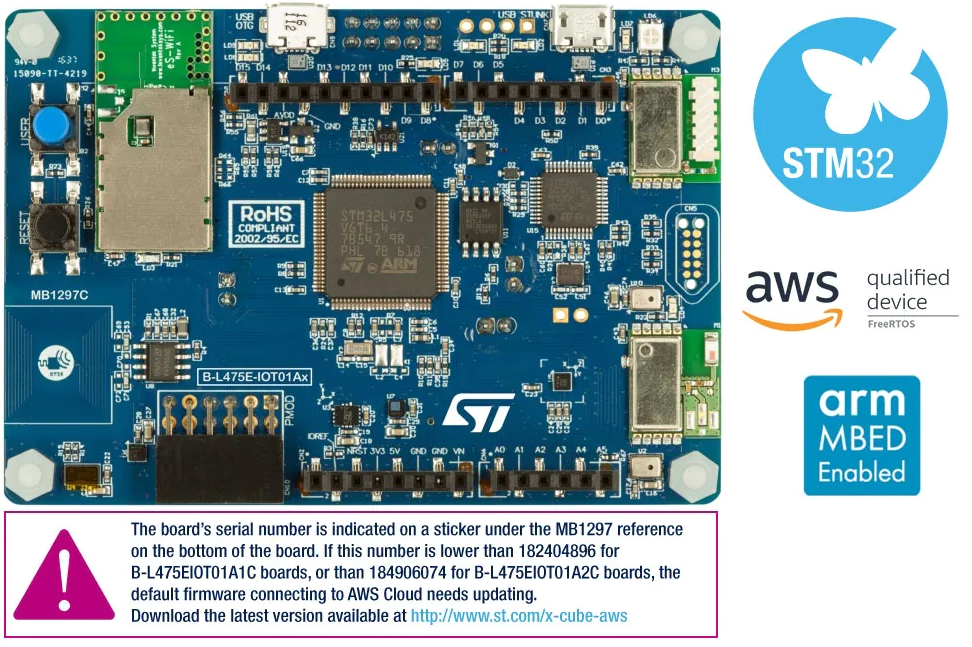
\includegraphics[scale=0.7]{Imagens/B-L475E-IOT01A2.png}
    \legend{Fonte: STMicroeletronics (2022).}
    \label{fig:B-L475E-IOT01A2}
\end{figure}

% -----------------------------------------------------------------------------
% Capítulo 3.3 - Criação de um nó IoT na rede AWS
% -----------------------------------------------------------------------------
\section{Criação de um nó IoT na rede AWS}\label{section:criacao_de_um_no_iot_na_rede_aws}

Um nó IoT é representado na AWS como uma coisa no serviço AWS IoT. Cada coisa, ou grupo de coisas, pertence a alguma região da AWS. Assim, o dispositivo de protótipo foi autenticado na região \textit{us-east-1} (N. Virginia) como \textit{B-L475E-IOT01A2}. O processo completo de criação, autenticação e autorização de uma coisa no AWS IoT se encontra na \autoref{section:criacao_de_uma_coisa_no_aws_iot}.

Para que o dispositivo tenha permissões de acesso a recursos da AWS, um certificado atrelado a uma política foi criado. Essa política da permissões de conexão, publicação, inscrição, e recebimento de tópicos MQTT ao dispositivo e pode ser vista no \autoref{lst:bl475e_policy}.

\begin{lstlisting}[float=htbp,language=json,firstnumber=1,caption={Política dando permissões de conexão, publicação, inscrição, e recebimento de tópicos MQTT ao dispositivo \textit{B-L475E-IOT01A2}.},label=lst:bl475e_policy]
{
  "Version": "2012-10-17",
  "Statement": [
    {
      "Effect": "Allow",
      "Action": "iot:Connect",
      "Resource": "arn:aws:iot:us-east-1:332527922592:*"
    },
    {
      "Effect": "Allow",
      "Action": "iot:Publish",
      "Resource": "arn:aws:iot:us-east-1:332527922592:*"
    },
    {
      "Effect": "Allow",
      "Action": "iot:Subscribe",
      "Resource": "arn:aws:iot:us-east-1:332527922592:*"
    },
    {
      "Effect": "Allow",
      "Action": "iot:Receive",
      "Resource": "arn:aws:iot:us-east-1:332527922592:*"
    }
  ]
}
\end{lstlisting}

Ao final do processo, o AWS IoT permite que o usuário faça \textit{download} dos certificados de autenticação e autorização gerados. Esses certificados devem ser carregados no protótipo, dando permissões ao dispositivo de acesso aos serviços do AWS IoT e permitindo a sua identificação por parte da AWS.

% -----------------------------------------------------------------------------
% Capítulo 3.4 - Estabelecendo conexão entre o protótipo e o AWS IoT
% -----------------------------------------------------------------------------
\section{Estabelecendo conexão entre o protótipo e o AWS IoT}\label{section:estabelecendo_conexao_entre_o_prototipo_e_o_aws_iot}

Para estabelecer conexão entre o protótipo e o AWS IoT, através do protocolo MQTT, alguns projetos de exemplo disponibilizados pela STMicroelectronics e pelo Amazon FreeRTOS foram utilizados. Destaca-se os projetos \textit{aws-demos} e o \textit{B-L475E-IOT01-AWS}.

O projeto de exemplo \textit{B-L475E-IOT01-AWS} é disponibilizado dentro do pacote expansão do software AWS IoT para STM32Cube, fornecido pela STMicroelectronics. Esse pacote está disponível para \textit{download} no link \href{https://www.st.com/content/st_com/en/products/embedded-software/mcu-mpu-embedded-software/stm32-embedded-software/stm32cube-expansion-packages/x-cube-aws.html}{AWS IoT software expansion for STM32Cube}. Nesse exemplo, o dispositivo se conecta ao AWS IoT com as credenciais carregadas via USB. Quando o botão do usuário é pressionado, um comando de alternância de LED é enviado para o IoT \textit{endpoint}, que retorna a mensagem para a placa e aciona a alternância do LED. Os dados de sensores da placa também são coletados e publicados na nuvem a cada 10 segundos.

A aplicação envia o comando de alternância do estado do LED para o tópico MQTT "\$aws/things/B-L475E-IOT01A2/shadow/update" e segue o formato JSON apresentado no \autoref{lst:set_led_state}.

\begin{lstlisting}[float=htbp,language=json,firstnumber=1,caption={Formato da mensagem de alternância do estado do LED.},label=lst:set_led_state]
{
    "state": {
        "desired": {
            "LED_value": "On"
        }
    }
}
\end{lstlisting}

O canal oficial da STMicroelectronics no YouTube disponibiliza um vídeo demonstrando o projeto sendo executado. O vídeo está disponível no link \href{https://www.youtube.com/watch?v=6eUqxjBL_wI}{Getting starting with STM32L4 Discovery kit IoT node}.

\textbf{Notas}:
\begin{alineas}
    \item O projeto de exemplo está disponível para o kit de desenvolvimento \textit{B-L475E-IOT01} somente para a versões 1.2.1, 1.4.0 e 1.4.1;
    \item O projeto conta com um arquivo binário que pode ser diretamente carregado no kit;
    \item O projeto possui problemas de compilação quando executado no sistema operacional Windows. Para solucionar os erros de compilação, o usuário deve substituir alguns caminhos relativos no \textit{script} de compilação por caminhos completos.
\end{alineas}

Para fins de prototipagem, o exemplo disponibilizado pela STMicroelectronics atendeu as necessidades do projeto e foi utilizado no processo de validação. Dessa forma, após a configuração do protótipo e autenticação no AWS IoT, a conexão via MQTT foi estabelecida.

% -----------------------------------------------------------------------------
% Capítulo 3.5 - Criação de Habilidades com o Alexa Skills Kit
% -----------------------------------------------------------------------------
\section{Criação de Habilidades com o \textit{Alexa Skills Kit}}

Para a criação de uma habilidade na Amazon Alexa, fez-se uso do ASK e do Console do Desenvolvedor Alexa. A Amazon sugere que o desenvolvimento de uma habilidade ocorra seguindo os seguintes passos:

\begin{enumerate}
    \item Criação de um nome para a habilidade;
    \item Criação de Intenções, amostras e Slots;\label{enum:criacao_de_intencoes_amostras_e_slots}
    \item Compilação do modelo;
    \item Definição de um \textit{endpoint} para o gerenciamento de requisições feitas pelo usuário;\label{enum:definicao_de_endpoint}
    \item Produtização e monetização da habilidade.
\end{enumerate}

O nome da habilidade foi definido como \textit{B-L475E-IOT01A2-Skill}. Os itens \autoref{enum:criacao_de_intencoes_amostras_e_slots} e \autoref{enum:definicao_de_endpoint} constituem o \textit{frontend} e o \textit{backend} da habilidade, respectivamente.

% -----------------------------------------------------------------------------
% Capítulo 3.5.1 - Frontend da habilidade B-L475E-IOT01A2-Skill
% -----------------------------------------------------------------------------
\subsection{\textit{Frontend} da habilidade \textit{B-L475E-IOT01A2-Skill}}\label{subscrion:frontend_bl475eiot01a2_skill}

O ASK permite que o desenvolvimento do \textit{frontend} aconteça via interface web e/ou arquivo JSON. O código que define o \textit{frontend} da aplicação pode ser encontrada no seguinte repositório git: \href{https://docs.aws.amazon.com/codecommit/latest/userguide/setting-up-ide-vs.html}{guiguitz/PENDING}. Um trecho do código está disponibilizado no \autoref{lst:frontend_bl475eiot01a2_skill}.

\begin{lstlisting}[float=htbp,language=json,firstnumber=1,caption={Trecho do arquivo JSON que descreve o \textit{frontend} da habilidade \textit{B-L475E-IOT01A2-Skill}.},label=lst:frontend_bl475eiot01a2_skill]
{
// ...
  "invocationName": "my node thing",
  "intents": [
    {
      "name": "HelloWorldIntent",
      "slots": [],
      "samples": [
        "good morning",
        "hello"
      ]
    },
    {
      "name": "SetLedStateIntent",
      "slots": [
        {
          "name": "ON_OFF_SLOT",
          "type": "ON_OFF_SLOT"
        }
      ],
      "samples": [
        "set led {ON_OFF_SLOT}",
        "turn led {ON_OFF_SLOT}",
      ]
    }
  ],
  "types": [
    {
      "name": "ON_OFF_SLOT",
      "values": [
        {
          "name": {
            "value": "OFF"
          }
        },
        {
          "name": {
            "value": "ON"
          }
        }
      ]
    }
  ]
// ...
}
\end{lstlisting}

% -----------------------------------------------------------------------------
% Capítulo 3.5.2 - Backend da habilidade B-L475E-IOT01A2-Skill
% -----------------------------------------------------------------------------
\subsection{\textit{Backend} da habilidade \textit{B-L475E-IOT01A2-Skill}}\label{subscrion:backend_bl475eiot01a2_skill}

Para o desenvolvimento do \textit{backend}, optou-se por estender as funcionalidades do ASK através de funções no AWS Lambda. Dessa forma, o desenvolvimento pode acontecer em Node.js, Python etc, assim como foi mencionado na \autoref{section:aws_lambda}. Para esse projeto, escolheu-se Python e \textit{ask-sdk} como linguagem de desenvolvimento e pacote SDK, respectivamente. \textit{ask-sdk} é o pacote referência para o desenvolvimento com o ASK. A função hospedada no AWS Lambda foi nomeada \textit{B-L475E-IOT01A2-Handler} e pode ser encontrada no seguinte repositório git: \href{https://github.com/guiguitz/B-L475E-IOT01A2-Handler}{guiguitz/B-L475E-IOT01A2-Handler}.

A função Lambda é orientada a eventos, assim como já foi explicado na \autoref{section:aws_lambda} e segue o diagrama de estados apresentado na \autoref{fig:diagrama_de_estados_bl475eiot01a2_handler}. Em termos práticos, após o acionamento da intenção \textit{SetLedStateIntent} através das frases "set led on", "set led off", "turn led on" e "set led off", função \textit{B-L475E-IOT01A2-Handler} envia uma mensagem para o tópico MQTT "\$aws/things/B-L475E-IOT01A2/shadow/update" que segue o formato apresentado no \autoref{lst:set_led_state}.

\begin{figure}[htbp]
  \centering
  \caption{Diagrama de estados da função \textit{B-L475E-IOT01A2-Handler}.}
  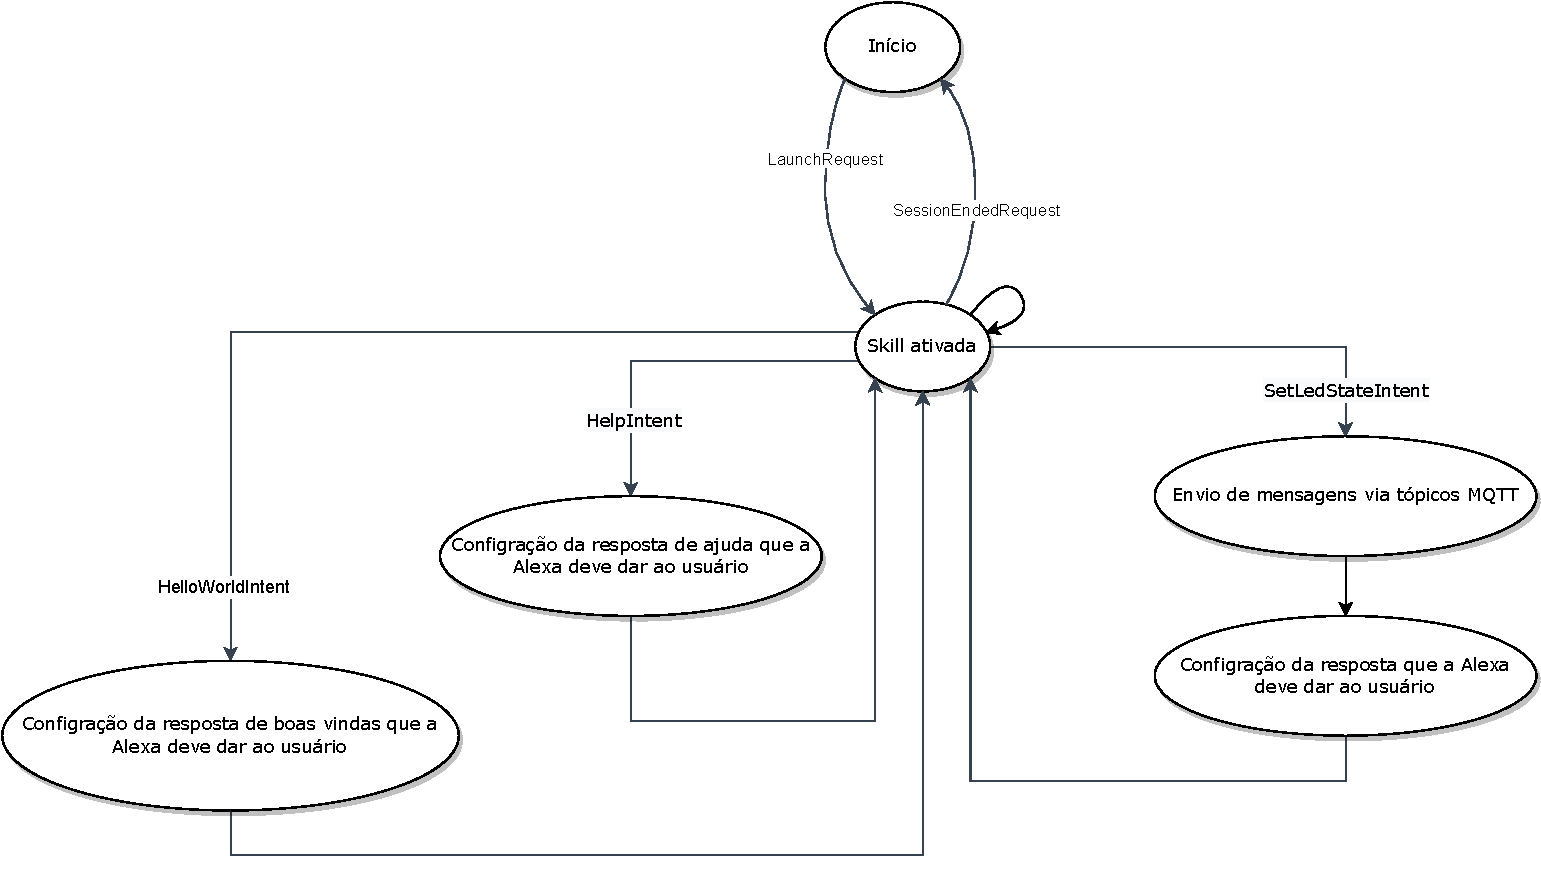
\includegraphics[scale=0.61]{Imagens/diagrama_de_estados_bl475eiot01a2_handler.pdf}
  \legend{Fonte: Produzido pelo autor (2022).}
  \label{fig:diagrama_de_estados_bl475eiot01a2_handler}
\end{figure}


% -----------------------------------------------------------------------------
% Capítulo 4 - Resultados e Discussão
% -----------------------------------------------------------------------------
\chapter{Resultados e Discussão}\label{chapter:resultados_e_discussoes}

PENDING...


% -----------------------------------------------------------------------------
% Capítulo 5 - Conclusões
% -----------------------------------------------------------------------------
\chapter{Conclusões}\label{chapter:conclusoes}

Conclui-se nesse trabalho que o kit de desenvolvimento \textit{B-L475E-IOT01A2} da STMicroelectronics atende os requisitos mínimos para a prototipagem de um nó IoT integrado ao serviço AWS IoT. Ademais, a infraestrutura de serviços da Amazon satisfaz as necessidades de um desenvolvedor de aplicações IoT dado que a AWS oferece os seguintes recursos a seus clientes:

\begin{itemize}
	\item Segurança com o modelo compartilhado de responsabilidade e o IAM.;
	\item Suporte para a criação de nós IoT com o serviço AWS IoT;
	\item Suporte de desenvolvimento e testes para o protocolo MQTT;
	\item Gerenciamento de dispositivos, ou conjunto de dispositivos, via AWS IoT Core;
	\item Pagamento somente do que for utilizado, reduzindo custos e permitindo crescimento em escala.
\end{itemize}

Conclui-se, também, que o desenvolvimento de habilidades para a Alexa através do ASK atende as necessidade dos desenvolvedores, uma vez a Amazon provem recursos para teste, SDKs para o desenvolvimento, suporte à CLI e possibilidade de implementação do back-end na própria AWS (através do AWS Lambda).

\section{Sugestão de Trabalhos Futuros}\label{section:sugesto_de_trabalhos_futuros}

Uma sugestão de trabalho futuro é a implementação de uma Alexa integrada no dispositivo \textit{B-L475E-IOT01A2}. Esse kit de desenvolvimento atende todos os parâmetros mínimos definidos pela Amazon para um dispositivo de IoT integrado à AVS (definidos na \autoref{table:reduced_hardware_footprint}). Um possível diagrama do projeto para esse trabalho futuro foi apresentado na \autoref{fig:integracao_avs_aws_iot}.

Outra sugestão de trabalho futuro é a implementação do suporte a outras linguagens, como o português e o italiano, para a habilidade \textit{B-L475E-IOT01A2-Skill}.

Por fim, outro trabalho importante é a produtização da habilidade \textit{B-L475E-IOT01A2}. A produtização de habilidades permite que usuários tenham acesso aos recursos dessa tecnologia em seus dispositivos Alexa após o \textit{download} na loja de habilidades da Amazon.

A série de vídeos \href{https://www.youtube.com/playlist?list=PLdZn93YfA_1ZP1WFkz6bm08v3zFfWwfGW}{Zero to Hero: Alexa Skills}, hospedada no canal \href{https://www.youtube.com/@AlexaDevelopers}{Alexa Developers} \nocite{ref:045}, demonstra como adicionar funcionalidades à habilidades Alexa. Os vídeos \href{https://www.youtube.com/watch?v=NXVmHWZZcjw&list=PLdZn93YfA_1ZP1WFkz6bm08v3zFfWwfGW&index=2}{Part 2: Skill Internationalization (i18n), Interceptors \& Error Handling} \nocite{ref:046} e \href{https://www.youtube.com/watch?v=I0fxuQQkLYg&list=PLdZn93YfA_1ZP1WFkz6bm08v3zFfWwfGW&index=11}{Part 11: Publishing} \nocite{ref:047} mostram como adicionar novas linguagens à habilidades Alexa e o processo de publicação, respectivamente.


% -----------------------------------------------------------------------------
% ELEMENTOS PÓS-TEXTUAIS
% -----------------------------------------------------------------------------
\postextual

% -----------------------------------------------------------------------------
% Referências bibliográficas
% -----------------------------------------------------------------------------
% \bibliographystyle{plain}
% \begin{small}
% \bibliography{Referências/referencias_zotero}
% \end{small}

% -----------------------------------------------------------------------------
% Apêndice
% -----------------------------------------------------------------------------
\chapter{Apêndice}\label{chapter:apendice}

% -----------------------------------------------------------------------------
% Capítulo X.1 - Kits de Desenvolvimento
% -----------------------------------------------------------------------------
\section{Kits de Desenvolvimento}\label{section:kits_de_desenvolvimento}

\begin{table}[htbp]
    \begin{tblr}{@{}|X[c,valign=m,gray!30]|X[c,valign=m]|X[c,valign=m]|X[c,valign=m]|X[c,valign=m]|X[c,valign=m]|@{}}
        \hline
        \textbf{Número de produto}        & B-L475E-IOT01A2                                                           & CORE-V MCU DevKit                                                   & SLN-ALEXA-IOT                                  \\ \hline
        \textbf{Descrição}                & STM32L4 Discovery kit Nó IoT, low-power wireless, BLE, NFC, SubGHz, Wi-Fi & European RISC-V chip for IoT development kit                        & EdgeReady MCU Based Solution for Alexa for IOT \\ \hline
        \textbf{Processador}              & Arm® Cortex®-M4                                                           & CV32E40P processor core                                             & Arm® Cortex®-M7 Core                           \\ \hline
        \textbf{FreeRTOS}                 & Sim                                                                       & Não Disponível                                                      & Sim                                            \\ \hline
        \textbf{Conectividade}            & Inventek ISM43362 Wi-Fi Module                                            & Espressif AWS IoT ExpressLink Module for AWS IoT cloud interconnect & Bluetooth LE 4.2, 802.11 b/g/n Wi-Fi®          \\ \hline
        \textbf{Microfones}               & 2 digital omnidirectional microphones (MP34DT01)                          & Não Disponível                                                      & Digital MEMS microphones (x3)                  \\ \hline
        \textbf{Alto-falante}             & Não Disponível                                                            & Não Disponível                                                      & Não Disponível                                 \\ \hline
        \textbf{Preço nas Lojas Oficiais} & \$53,00                                                                   & Preços Individuais                                                  & \$171,35                                       \\ \hline
    \end{tblr}
    \caption{kits de desenvolvimento recomendados pela Amazon para o desenvolvimento de aplicações IoT (A).}
    \label{table:development_kit_a}
\end{table}

\begin{table}[htbp]
    \begin{tblr}{@{}|X[c,valign=m,gray!30]|X[c,valign=m]|X[c,valign=m]|X[c,valign=m]|X[c,valign=m]|X[c,valign=m]|@{}}
        \hline
        \textbf{Número de produto}        & Home Hub 100 Dev Kit for Amazon AVS                                                                                                                                             & STEVAL-VOICE-UI                                                                                                                                                            \\ \hline
        \textbf{Descrição}                & A hardware and software development kit with multi-core connectivity designed to support AVS for AWS IoT Core connected devices                                                 & Qualified hardware reference design enabling easy and cost effective addition of the Alexa Voice Service (AVS) Integration for AWS IoT core to your smart embedded devices \\ \hline
        \textbf{Processador}              & Arm Cortex-M4F CPU                                                                                                                                                              & Dual Arm® Cortex®-A7 and Cortex®-M4 Cores                                                                                                                                  \\ \hline
        \textbf{FreeRTOS}                 & Sim                                                                                                                                                                             & Sim                                                                                                                                                                        \\ \hline
        \textbf{Conectividade}            & Integrated Bluetooth 5, Qualcomm® Bluetooth Mesh connectivity, low power Wi-Fi 802.11n in 2.4GHz/5GHz bands, and 802.15.4, with support for ZigBee3.0 and Thread via OpenThread & WIFI subsystem including Murata 1DX module used in bypass mode and ISSI IS25LP016D 2Mbytes NOR flash hosting WIFI low level software                                       \\ \hline
        \textbf{Microfones}               & Não Disponível                                                                                                                                                                  & 2 MP23DB01HP Microphone Mems                                                                                                                                               \\ \hline
        \textbf{Alto-falante}             & 1x                                                                                                                                                                              & 1x (8 ohm)                                                                                                                                                                 \\ \hline
        \textbf{Preço nas Lojas Oficiais} & £42.95                                                                                                                                                                          & \$248.75                                                                                                                                                                   \\ \hline
    \end{tblr}
    \caption{kits de desenvolvimento recomendados pela Amazon para o desenvolvimento de aplicações IoT (B).}
    \label{table:development_kit_b}
\end{table}

% -----------------------------------------------------------------------------
% Capítulo X.2 - Criação de uma coisa no AWS IoT
% -----------------------------------------------------------------------------
\section{Criação de uma coisa no AWS IoT}\label{section:criacao_de_uma_coisa_no_aws_iot}

SEQUÊNCIA DE PRINTSCREENS DURANTE A CRIAÇÃO DE UMA COISA NO AWS IOT!


\end{document}
